
\section{二维图类型}

{%
\tikzset{external/figure name/.add={}{twodim_}}

\PGFPlots{} 支持多种二维线图，例如分段线性线图、分段常值图、平滑图、
柱状图和梳状图。其中大多数直接使用 \PGF{} 的 plot handler 库，参见
\cite[Section~18.8]{tikz}。

图类型是绘图样式的一部分，因此通过选项来设置。大多数基本二维图类型
属于 \Tikz{}，参见 \cite[Section~18.8]{tikz}，\Tikz{} 用户可能已经
熟悉它们。这里也对它们进行文档说明。


\subsection{线性图}

\begin{plottype}{sharp plot}
    线性（"折线"）图是默认值。点坐标之间简单地用直线连接。
\begin{codeexample}[]
\begin{tikzpicture}
\begin{axis}
    \addplot+ [
        sharp plot,
    ] coordinates {
        (0,0) (1,2) (2,3)
    };
\end{axis}
\end{tikzpicture}
\end{codeexample}

    这里的 `|+|' 表示使用正常的绘图循环列表，并将 `|sharp plot|'
    附加到其选项列表中。
\end{plottype}


\subsection{平滑图}

\begin{plottype}{smooth}
    平滑图在相邻点之间进行平滑插值。
\begin{codeexample}[]
\begin{tikzpicture}
\begin{axis}
    \addplot+ [
        smooth,
    ] coordinates {
        (0,0) (1,2) (2,3)
    };
\end{axis}
\end{tikzpicture}
\end{codeexample}
\end{plottype}

正如~\cite{tikz} 中详细描述的那样，这个 plot handler 会产生一个
"平滑"的轮廓。然而，它"并不十分智能"（比较~\cite{tikz}），与常见的
基于绘图的插值方案无关。

\begin{key}{/tikz/tension=\marg{tension} (initially 0.55)}
    一个控制如何确定剩余自由度的参数：它控制平滑效果。较高的值会产生
    更"圆润"的角，而较低的值会产生尖角。

    详情请参阅~\cite{tikz}。
\end{key}


\subsection{常值图}

常值图绘制平行于 $x$ 轴的线来连接坐标。不连续的边可以绘制或不绘制，
标记可以放置在左端或右端。

\begin{plottype}{const plot}
    用水平线和竖直线连接所有点。标记放置在线段的左端，使绘图在所有
    数据点处右连续。

\begin{codeexample}[]
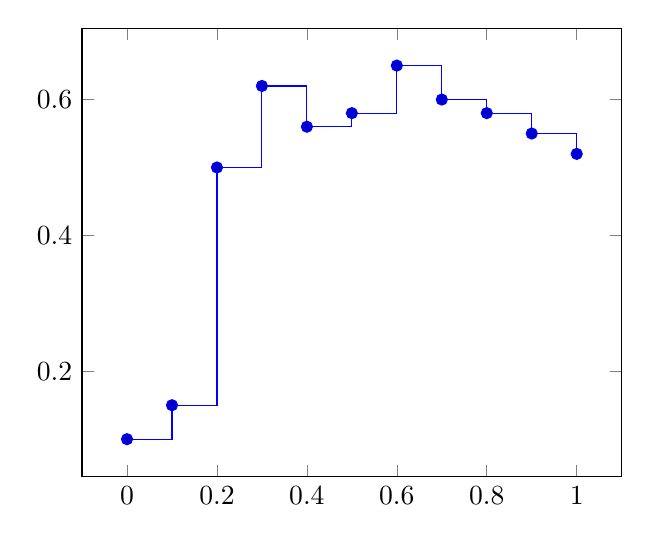
\begin{tikzpicture}
\begin{axis}
    \addplot+ [
        const plot,
    ] coordinates {
        (0,0.1)    (0.1,0.15)  (0.2,0.5)   (0.3,0.62)
        (0.4,0.56) (0.5,0.58)  (0.6,0.65)  (0.7,0.6)
        (0.8,0.58) (0.9,0.55)  (1,0.52)
    };
\end{axis}
\end{tikzpicture}
\end{codeexample}


\begin{codeexample}[]
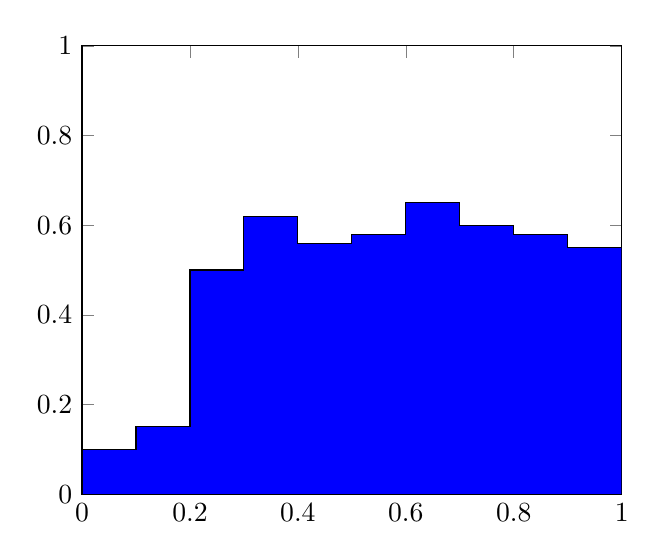
\begin{tikzpicture}
\begin{axis}[ymin=0,ymax=1,enlargelimits=false]
    \addplot [
        const plot,
        fill=blue,
        draw=black,
    ] coordinates {
        (0,0.1)    (0.1,0.15)  (0.2,0.5)   (0.3,0.62)
        (0.4,0.56) (0.5,0.58)  (0.6,0.65)  (0.7,0.6)
        (0.8,0.58) (0.9,0.55)  (1,0.52)
    }
        \closedcycle
    ;
\end{axis}
\end{tikzpicture}
\end{codeexample}
\end{plottype}

\begin{plottype}{const plot mark left}
    `|const plot|' 的别名。
\end{plottype}

\begin{plottype}{const plot mark right}
    一个变体，将标记放置在每个线段的右端，使绘图在给定坐标处左连续。
    %
\begin{codeexample}[]
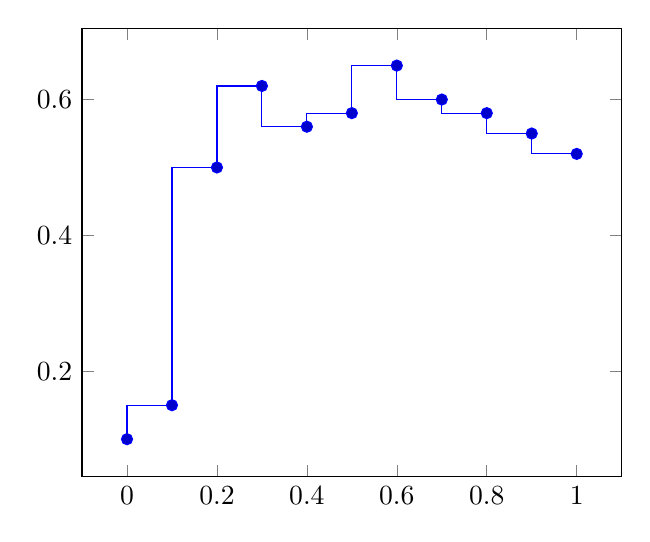
\begin{tikzpicture}
\begin{axis}
    \addplot+ [
        const plot mark right,
    ] coordinates {
        (0,0.1)    (0.1,0.15)  (0.2,0.5)   (0.3,0.62)
        (0.4,0.56) (0.5,0.58)  (0.6,0.65)  (0.7,0.6)
        (0.8,0.58) (0.9,0.55)  (1,0.52)
    };
\end{axis}
\end{tikzpicture}
\end{codeexample}
\end{plottype}

\begin{plottype}{const plot mark mid}
    一个变体，将标记放置在每个线段的中间，使绘图关于其数据点对称。
    %
\begin{codeexample}[]
\begin{tikzpicture}
\begin{axis}
    \addplot+ [
        const plot mark mid,
    ] coordinates {
        (0,0.1)    (0.1,0.15)  (0.2,0.5)   (0.3,0.62)
        (0.4,0.56) (0.5,0.58)  (0.6,0.65)  (0.7,0.6)
        (0.8,0.58) (0.9,0.55)  (1,0.52)
    };
\end{axis}
\end{tikzpicture}
\end{codeexample}
    %
    注意，"对称"仅对恒定的网格间距成立：如果相邻数据点之间的 $x$
    距离不同，|const plot mark mid| 会在每对连续点之间的中间位置绘制
    竖直线。
\end{plottype}

\begin{plottype}{jump mark left}
    `|const plot mark left|' 的一个变体，不绘制竖直线。
    %
\begin{codeexample}[]
\begin{tikzpicture}
\begin{axis}[samples=8]
    \addplot+ [
        jump mark left,
        domain=-5:0,
    ] {4*x^2 - 5};

    \addplot+ [
        jump mark right,
        domain=-5:0,
    ] {0.7*x^3 + 50};
\end{axis}
\end{tikzpicture}
\end{codeexample}
\end{plottype}

\begin{plottype}{jump mark right}
    `|const plot mark right|' 的一个变体，不绘制竖直线。
\end{plottype}

\begin{plottype}{jump mark mid}
    `|const plot mark mid|' 的一个变体，不绘制竖直线。
    %
\begin{codeexample}[]
\begin{tikzpicture}
\begin{axis}
    \addplot+ [
        jump mark mid,
    ] coordinates {
        (0,0.1)    (0.1,0.15)  (0.2,0.5)   (0.3,0.62)
        (0.4,0.56) (0.5,0.58)  (0.6,0.65)  (0.7,0.6)
        (0.8,0.58) (0.9,0.55)  (1,0.52)
    };
\end{axis}
\end{tikzpicture}
\end{codeexample}
\end{plottype}


\subsection{柱状图}

柱状图在坐标处放置水平或垂直的柱。同一坐标轴中的多个柱状图可以堆叠
在一起，也可以并排排列。

\begin{plottype}{xbar}
    在 $(y=0)$ 线与每个坐标之间放置水平柱。

    此选项按每个绘图单独使用，仅配置坐标的可视化方式。图级别的样式
    |/pgfplots/xbar| 还会为刻度、图例和多个绘图设置合理的选项。
    %
\begin{codeexample}[]
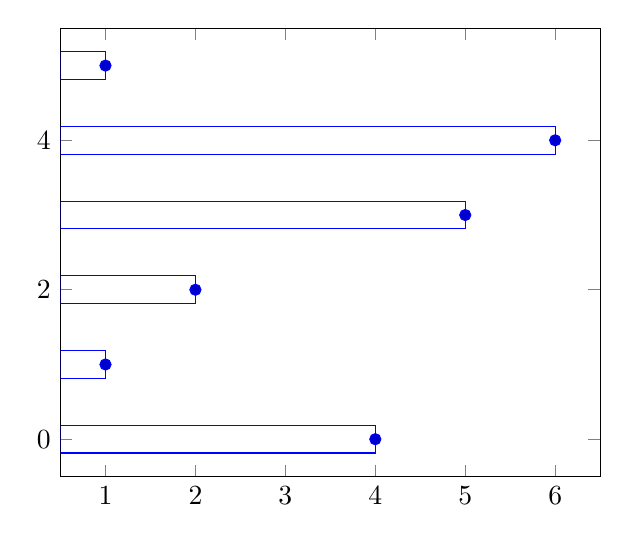
\begin{tikzpicture}
\begin{axis}
    \addplot+ [
        xbar,
    ] coordinates {
        (4,0) (1,1) (2,2)
        (5,3) (6,4) (1,5)
    };
\end{axis}
\end{tikzpicture}
\end{codeexample}
    %
    柱以绘图坐标为中心，宽度为 |bar width|。使用柱状图通常不仅仅意味着
    连接坐标的方式不同，例如将刻度绘制在坐标轴外侧、改变图例的外观，
    或者在出现多个 |\addplot| 命令时引入偏移。

    对于 |xbar|，有一个预配置的样式：如果你将 |xbar| 作为参数提供给
    坐标轴环境，它会自动安装并提供此功能。
    %
% \usetikzlibrary{patterns}
\begin{codeexample}[]
\begin{tikzpicture}
\begin{axis}[xbar,enlargelimits=0.15]
    \addplot [draw=blue,
        pattern=horizontal lines light blue,
    ] coordinates {
        (10,5) (15,10) (5,15) (24,20) (30,25)
    };
    \addplot [draw=black,
        pattern=horizontal lines dark blue,
    ] coordinates {
        (3,5) (5,10) (15,15) (20,20) (35,25)
    };
\end{axis}
\end{tikzpicture}
\end{codeexample}
    %
    这里 |xbar| 产生 |/pgfplots/xbar|，因为它是坐标轴的参数，
    而不是单个绘图的参数。

    对于柱状图，在柱附近提供文本坐标甚至描述性节点是很常见的。
    这可以分别使用 |symbolic y coords| 和 |nodes near coords| 键来实现：
    %
\begin{codeexample}[]
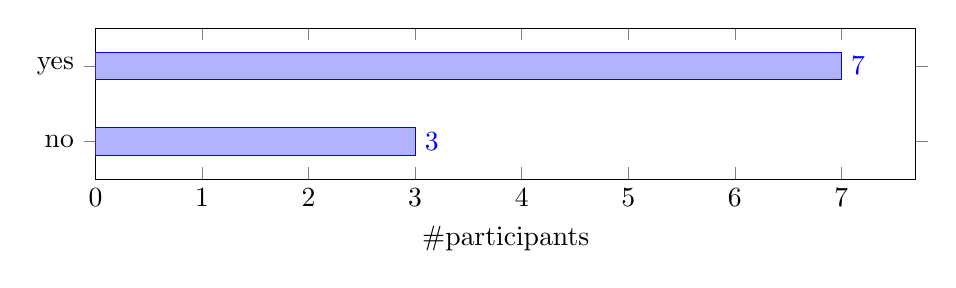
\begin{tikzpicture}
    \begin{axis}[
        xbar, xmin=0,
        width=12cm, height=3.5cm, enlarge y limits=0.5,
        xlabel={\#participants},
        symbolic y coords={no,yes},
        ytick=data,
        nodes near coords, nodes near coords align={horizontal},
    ]
        \addplot coordinates {(3,no) (7,yes)};
    \end{axis}
\end{tikzpicture}
\end{codeexample}
    %
    |symbolic y coords| 定义了一个可接受坐标的字典，这些坐标随后将作为
    $y$ 坐标使用；而 |nodes near coords| 键将值显示为额外的节点
    （详情参见它们的参考文档）。该示例使用了 |enlarge y limits| 以获得
    更多空闲空间，因为默认间距并不总是适合柱状图。

    注意，如上例中显式包含 |xmin=0| 可能相当重要。如果没有它，将使用
    下界：
    %
\begin{codeexample}[]
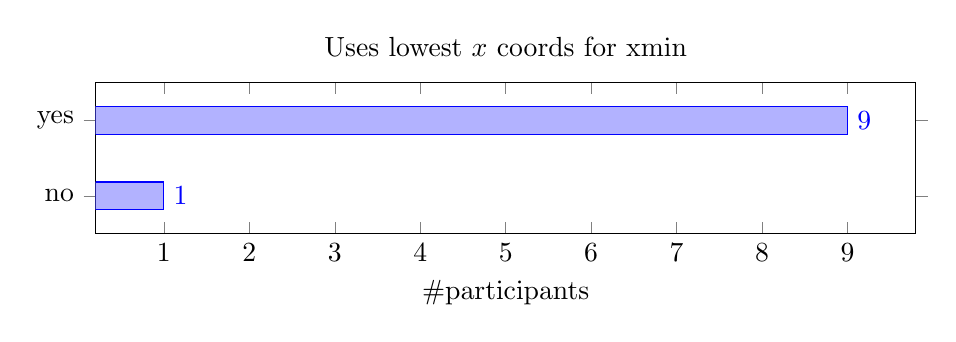
\begin{tikzpicture}
    \begin{axis}[
        title=Uses lowest $x$ coords for xmin,
        xbar,
        width=12cm, height=3.5cm, enlarge y limits=0.5,
        xlabel={\#participants},
        symbolic y coords={no,yes},
        ytick=data,
        nodes near coords, nodes near coords align={horizontal},
      ]
        \addplot coordinates {(1,no) (9,yes)};
    \end{axis}
\end{tikzpicture}
\end{codeexample}

    除了线、填充和颜色样式外，柱还可以用 |bar width| 和 |bar shift|
    进行配置，见下文。
\end{plottype}

\begin{stylekey}{/pgfplots/xbar=\marg{shift for multiple plots} (default 2pt)}
    此样式为整个坐标轴设置 |/tikz/xbar| \emph{以及}一些关于水平柱的常用
    选项。如果你将 |xbar| 作为坐标轴参数提供，这会自动完成，见上文。

    |xbar| 样式定义了当多个绘图放入同一坐标轴时的偏移。它将柱相邻绘制，
    彼此之间相隔 \meta{shift for multiple plots}。此外，它还设置了
    |bar cycle list| 样式，并设置了刻度和图例的外观选项。

    该样式定义如下。
    %
\begin{codeexample}[code only]
\pgfplotsset{
    /pgfplots/xbar/.style={
        /tikz/xbar,
        bar cycle list,
        tick align=outside,
        xbar legend,
        /pgfplots/bar shift auto={#1},
    },
}
\end{codeexample}

    \begin{pgfplotskey}{bar shift auto=\marg{shift for multiple plots} (default 2pt)}
        |bar shift| 的公式根据绘图总数和当前绘图的编号来分配偏移。
        它的设计目的是填充总宽度 $n \cdot $|bar width|$ + (n-1) \cdot $
        \meta{shift for multiple plots}。其中 $0.5$ 用于补偿居中。

        该样式定义为
        %
\begin{codeexample}[code only]
\pgfplotsset{
    /pgfplots/bar shift auto/.style={
        /pgf/bar shift={%
            % total width = n*w + (n-1)*skip
            % -> subtract half for centering
            -0.5*(\numplotsofactualtype*\pgfplotbarwidth + (\numplotsofactualtype-1)*(#1)) +
            % the '0.5*w' is for centering
            (.5+\plotnumofactualtype)*\pgfplotbarwidth + \plotnumofactualtype*(#1)},
    },
}
\end{codeexample}
    \end{pgfplotskey}
\end{stylekey}

\begin{plottype}{ybar}
    与 |xbar| 类似，此选项生成柱状图。它在 ($x=0$) 线与每个输入坐标
    之间绘制垂直柱。
    %
\begin{codeexample}[]
\begin{tikzpicture}
\begin{axis}
    \addplot+ [
        ybar,
    ] coordinates {
        (0,3) (1,2) (2,4) (3,1) (4,2)
    };
\end{axis}
\end{tikzpicture}
\end{codeexample}
    %
    上面的示例只是改变了输入坐标的可视化方式。正如 |xbar| 中提到的，
    通常需要为同一坐标轴中的多个柱修改图例和偏移。

    有一个预定义的样式，当提供给坐标轴环境时会安装这些自定义设置：
    %
\begin{codeexample}[]
\begin{tikzpicture}
\begin{axis}[
    x tick label style={
        /pgf/number format/1000 sep=},
    ylabel=Population,
    enlargelimits=0.15,
    legend style={at={(0.5,-0.15)},
        anchor=north,legend columns=-1},
    ybar,
    bar width=7pt,
]
    \addplot coordinates {
        (1930,50e6) (1940,33e6)
        (1950,40e6) (1960,50e6) (1970,70e6)
    };
    \addplot coordinates {
        (1930,38e6) (1940,42e6)
        (1950,43e6) (1960,45e6) (1970,65e6)
    };
    \addplot coordinates {
        (1930,15e6) (1940,12e6)
        (1950,13e6) (1960,25e6) (1970,35e6)
    };
    \addplot [red,line legend,
        sharp plot,update limits=false,
    ] coordinates { (1910,4.3e7) (1990,4.3e7) }
        node [above] at (1950,4.3e7) {Houses};

    \legend{Far,Near,Here,Annot}
\end{axis}
\end{tikzpicture}
\end{codeexample}
    %
    这里，|ybar| 产生 |/pgfplots/ybar|，因为它是坐标轴的参数，
    而不是单个绘图的参数。该样式影响前三个 |\addplot| 命令。注意它会
    在绘图坐标周围水平移动它们。第四个 |\addplot| 命令是某种注释，
    它不 |update limits|。

    |ybar| 样式可以以与 |xbar| 中描述类似的方式与 |symbolic x coords|
    结合使用：
    %
\begin{codeexample}[]
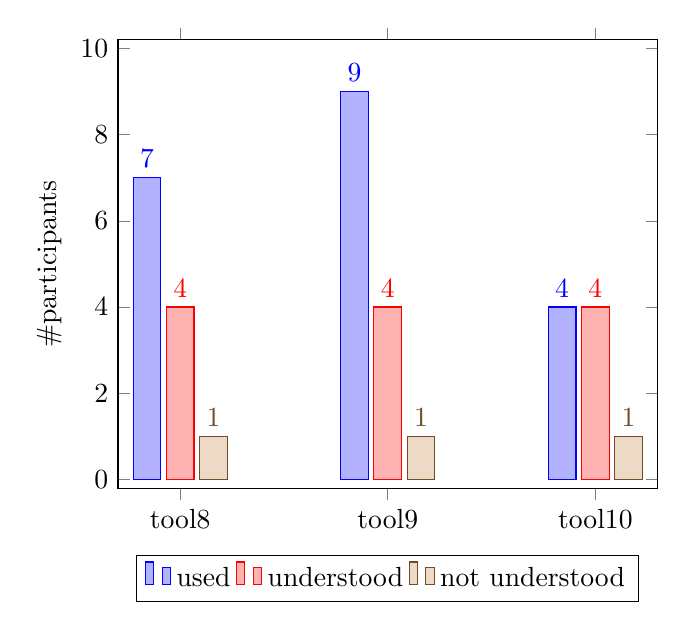
\begin{tikzpicture}
\begin{axis}[
    ybar,
    enlargelimits=0.15,
    legend style={at={(0.5,-0.15)},
    anchor=north,legend columns=-1},
    ylabel={\#participants},
    symbolic x coords={tool8,tool9,tool10},
    xtick=data,
    nodes near coords,
    nodes near coords align={vertical},
]
\addplot coordinates {(tool8,7) (tool9,9) (tool10,4)};
\addplot coordinates {(tool8,4) (tool9,4) (tool10,4)};
\addplot coordinates {(tool8,1) (tool9,1) (tool10,1)};
    \legend{used,understood,not understood}
\end{axis}
\end{tikzpicture}
\end{codeexample}

    与 |xbar| 一样，柱宽和偏移可以用 |bar width| 和 |bar shift| 配置。
    但是，柱偏移最好作为 |/pgfplots/ybar| 的参数提供，因为该样式会
    覆盖柱偏移。因此，优先使用 |/pgfplots/ybar=4pt| 来设置柱偏移。

    有时，直接在柱附近写出 $y$ 值会很有用。这可以使用 |nodes near coords|
    方法来实现：
    %
\begin{codeexample}[]
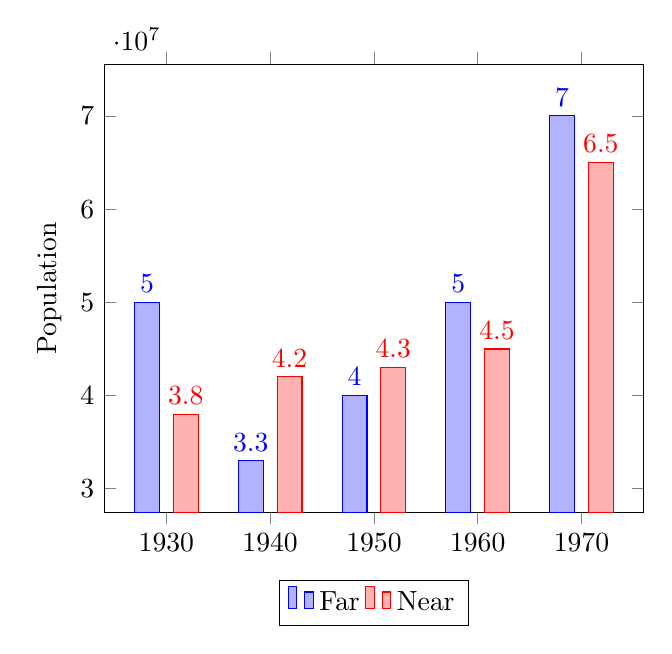
\begin{tikzpicture}
\begin{axis}[
    x tick label style={
        /pgf/number format/1000 sep=},
    ylabel=Population,
    enlargelimits=0.15,
    legend style={at={(0.5,-0.15)},
        anchor=north,legend columns=-1},
    ybar=5pt,% configures `bar shift'
    bar width=9pt,
    nodes near coords,
    point meta=y *10^-7, % the displayed number
]
    \addplot coordinates {
        (1930,50e6) (1940,33e6)
        (1950,40e6) (1960,50e6) (1970,70e6)
    };
    \addplot coordinates {
        (1930,38e6) (1940,42e6)
        (1950,43e6) (1960,45e6) (1970,65e6)
    };
    \legend{Far,Near}
\end{axis}
\end{tikzpicture}
\end{codeexample}

    当然，任何辅助样式的修改都是可能的。柱状图的一个有用示例可能是
    使用旋转的刻度标签：
    %
\begin{codeexample}[]
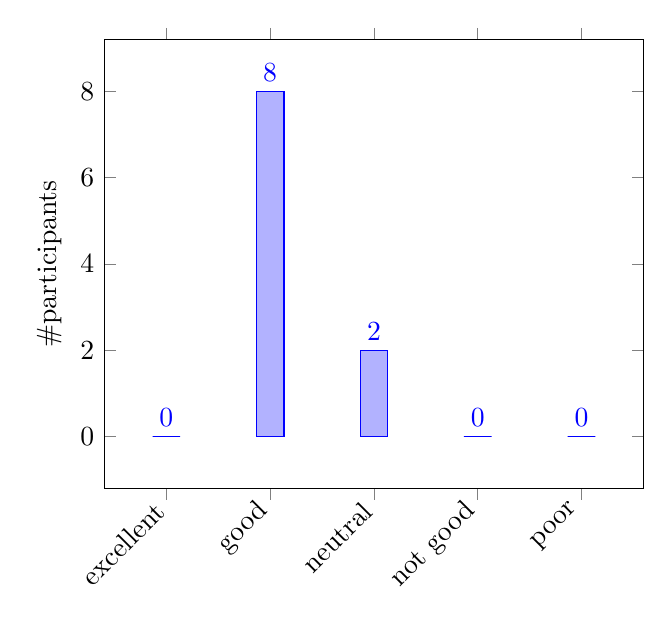
\begin{tikzpicture}
\begin{axis}[
    ybar,
    enlargelimits=0.15,
    legend style={at={(0.5,-0.2)},
    anchor=north,legend columns=-1},
    ylabel={\#participants},
    symbolic x coords={excellent,good,neutral,%
        not good,poor},
    xtick=data,
    nodes near coords,
    nodes near coords align={vertical},
    x tick label style={rotate=45,anchor=east},
]
    \addplot coordinates {
        (excellent,0) (good,8) (neutral,2)
        (not good,0) (poor,0)
    };
\end{axis}
\end{tikzpicture}
\end{codeexample}
\end{plottype}

\begin{stylekey}{/pgfplots/ybar=\marg{shift for multiple plots} (default 2pt)}
    与 |/pgfplots/xbar| 类似，此样式设置 |/tikz/ybar| 选项来绘制
    垂直柱状图，同时它还提供了垂直柱状图的常用选项。

    如果在 axis 环境中提供 |ybar|，则会选择 |/pgfplots/ybar|
    而不是 |/tikz/ybar|。

    它会修改图例、将刻度绘制到坐标轴线外侧，并将多个 |\addplot|
    参数彼此相邻绘制；这些柱以 $x$-坐标为中心，并由 \meta{shift for multiple plots}
    分隔。它还会为 |every node near coord| 安装 |bar shift|。此外，它
    安装 |bar cycle list| 样式。它的定义方式与
    |/pgfplots/xbar| 类似。
\end{stylekey}

\begin{pgfplotskey}{bar cycle list}
    一个为多个柱状图安装循环列表的样式。
    %
\begin{codeexample}[code only]
\pgfplotsset{
    /pgfplots/bar cycle list/.style={/pgfplots/cycle list={
            {blue,fill=blue!30!white,mark=none},
            {red,fill=red!30!white,mark=none},
            {brown!60!black,fill=brown!30!white,mark=none},
            {black,fill=gray,mark=none},
        },
    },
}
\end{codeexample}
\end{pgfplotskey}

\begin{key}{/pgf/bar width=\marg{dimension or unit} (initially 10pt)}
    配置 |xbar| 和 |ybar| 使用的宽度。允许提供数学表达式。

    从 \PGFPlots{} 1.7 开始，允许将 \emph{单位} 作为 |bar width|
    提供。在这种情况下，|bar width| 将被解释为坐标轴单位：
    %
\begin{codeexample}[]
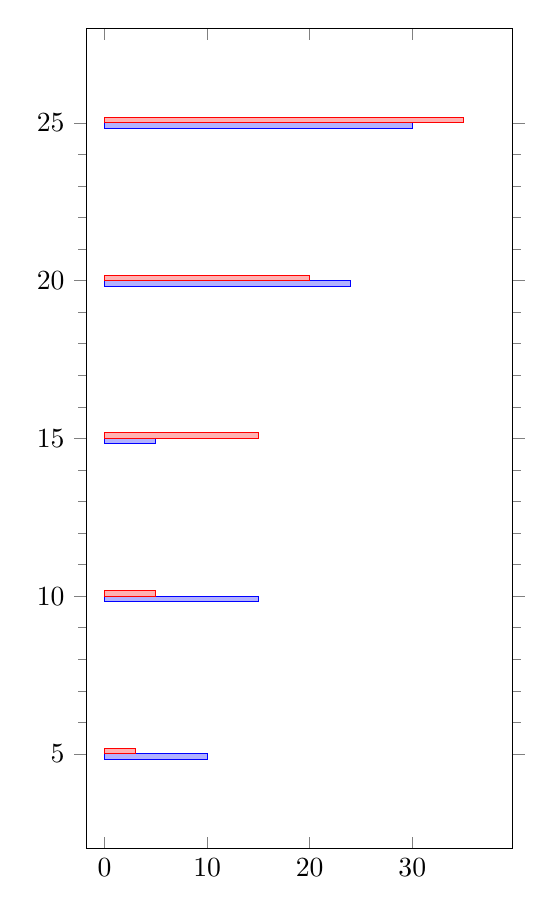
\begin{tikzpicture}
\begin{axis}[
    xbar=0pt,% space of 0pt between adjacent bars
    bar width=2,
    width=7cm,
    height=12cm,
    minor y tick num=4,
    ytick=data,
    enlargelimits=0.15,
]
    \addplot coordinates {
        (10,5) (15,10) (5,15) (24,20) (30,25)
    };
    \addplot coordinates {
        (3,5) (5,10) (15,15) (20,20) (35,25)
    };
\end{axis}
\end{tikzpicture}
\end{codeexample}
    %
    为了将参数解释为单位，你必须在导言区写入
    |\pgfplotsset{compat=1.7}|（或更新版本）。较旧的版本会在参数不是
    尺寸时隐式地追加 |pt| 后缀。

    \begin{command}{\pgfplotbarwidth}
        一个数学表达式，其结果为 |bar width| 的完全计算值
        （即包含任何单位计算）。
    \end{command}

    注意，你可能需要 |enlargelimits| 才能看到完整的柱——\PGFPlots{}
    不会自动更新坐标轴范围以适配 |bar width|。
\end{key}

\begin{key}{/pgf/bar shift=\marg{dimension or unit} (initially 0pt)}
    配置 |xbar| 和 |ybar| 的偏移。将 |bar shift| 与 |bar width|
    一起使用，即可在同一坐标轴中绘制多个柱状图。允许提供数学表达式。

    从 \PGFPlots{}~1.7 开始，允许将 \emph{单位} 作为 |bar shift|
    提供。在这种情况下，|bar shift| 将被解释为坐标轴单位。

    \begin{command}{\pgfplotbarshift}
        一个数学表达式，其结果为 |bar shift| 的完全计算值
        （即包含任何单位计算）。
    \end{command}

    注意，你可能需要 |enlargelimits| 才能看到完整的柱——\PGFPlots{}
    不会自动更新坐标轴范围以适配 |bar shift|。
\end{key}

\begin{pgfplotskey}{bar direction=\mchoice{auto,x,y} (initially auto)}
    如果 \PGFPlots{} 遇到值 |bar width=1|（即\emph{没有}像 |1pt|
    这样的尺寸），它会尝试评估柱的方向。

    默认配置 \declareandlabel{auto} 假设你写的是类似 |ybar,bar width=1|
    的东西。在这种情况下，很明显你有一个 $y$ 柱，\PGFPlots{} 会假设
    |bar direction=y|。

    但是，如果此上下文信息不可用，你可以在 \PGFPlots{} 不知道它
    处理的是 |xbar| 图时使用选项 \declaretext{x}，或者在 \PGFPlots{}
    不知道你指的是 |ybar| 图时使用 \declaretext{y}。
\end{pgfplotskey}

\begin{plottype}{ybar interval}
    此图类型生成宽度（和偏移）相对于坐标间隔的垂直柱。

    使用间隔时有一个概念上的不同：一个间隔由\emph{两个}坐标定义。
    由于 |ybar| 每个间隔有一个值，第 $i$ 个柱由以下内容定义
    %
    \begin{enumerate}
        \item 第 $i$ 个坐标的 $y$ 值，
        \item 第 $i$ 个坐标的 $x$ 值作为左边界，
        \item 第 $(i+1)$ 个坐标的 $x$ 值作为右边界。
    \end{enumerate}
    %
    因此，坐标\emph{多了一个}：最后一个坐标\emph{仅}用于确定间隔
    宽度；它的 $y$ 值不影响柱的外观。

    它按每个绘图单独安装，\emph{仅}配置坐标的可视化方式。参见样式
    |/pgfplots/ybar interval|，它配置整个图的外观。
    %
\begin{codeexample}[]
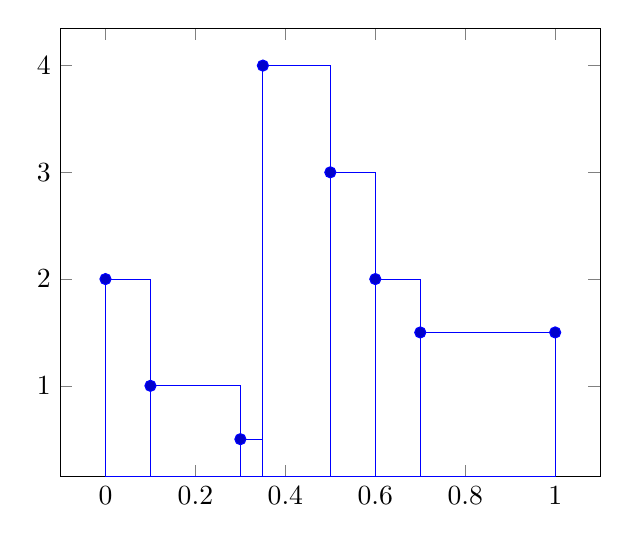
\begin{tikzpicture}
\begin{axis}
    \addplot+ [
        ybar interval,
    ] coordinates {
        (0,2) (0.1,1) (0.3,0.5) (0.35,4) (0.5,3)
        (0.6,2) (0.7,1.5) (1,1.5)
    };
\end{axis}
\end{tikzpicture}
\end{codeexample}

\begin{codeexample}[]
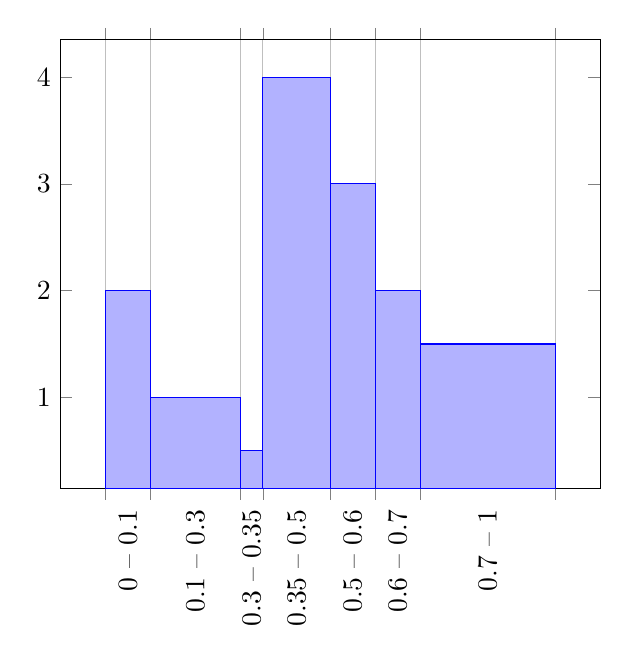
\begin{tikzpicture}
\begin{axis}[ybar interval,
    xtick=data,
    xticklabel interval boundaries,
    x tick label style={
        rotate=90,
        anchor=east,
    },
]
    \addplot coordinates {
        (0,2) (0.1,1) (0.3,0.5) (0.35,4) (0.5,3)
        (0.6,2) (0.7,1.5) (1,1.5)
    };
\end{axis}
\end{tikzpicture}
\end{codeexample}

\begin{codeexample}[]
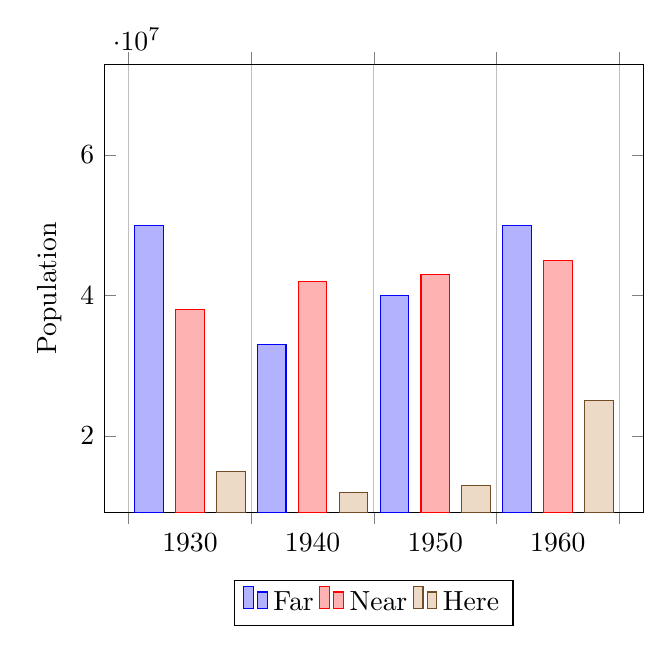
\begin{tikzpicture}
\begin{axis}[
    x tick label style={
        /pgf/number format/1000 sep=},
    ylabel=Population,
    enlargelimits=0.05,
    legend style={at={(0.5,-0.15)},
    anchor=north,legend columns=-1},
    ybar interval=0.7,
]
    \addplot coordinates {
        (1930,50e6) (1940,33e6)
        (1950,40e6) (1960,50e6) (1970,70e6)
    };
    \addplot coordinates {
        (1930,38e6) (1940,42e6)
        (1950,43e6) (1960,45e6) (1970,65e6)
    };
    \addplot coordinates {
        (1930,15e6) (1940,12e6)
        (1950,13e6) (1960,25e6) (1970,35e6)
    };
    \legend{Far,Near,Here}
\end{axis}
\end{tikzpicture}
\end{codeexample}
\end{plottype}

\begin{stylekey}{/pgfplots/ybar interval=\marg{relative width} (default 1)}
    一个用于为整个图安装 |ybar interval| 选项的样式。这包括刻度和图例
    的外观、同一图中多个柱状图的管理，以及使用 |bar cycle list| 样式
    的更合适的 |cycle list|。
\end{stylekey}

\begin{plottype}{xbar interval}
    与 |ybar interval| 类似，只是用于水平柱。
    %
\begin{codeexample}[]
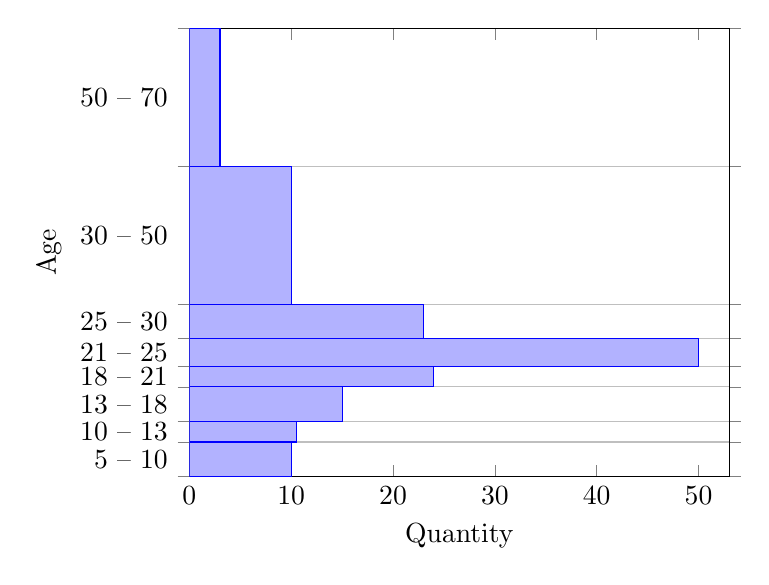
\begin{tikzpicture}
\begin{axis}[
    xmin=0,xmax=53,
    ylabel=Age,
    xlabel=Quantity,
    enlargelimits=false,
    ytick=data,
    yticklabel interval boundaries,
    xbar interval,
]
    \addplot coordinates {
        (10,5) (10.5,10) (15,13) (24,18) (50,21)
        (23,25) (10,30) (3,50) (3,70)
    };
\end{axis}
\end{tikzpicture}
\end{codeexample}
\end{plottype}

\begin{stylekey}{/pgfplots/xbar interval=\marg{relative width} (default 1)}
    一个用于为整个图安装 |xbar interval| 选项的样式，详情参见样式
    |/pgfplots/ybar interval|。
\end{stylekey}

\begin{pgfplotsxykey}{\x ticklabel interval boundaries}
    这些是样式键，用于设置 |x tick label as interval|（详情参见
    第\pageref{key:pgfplots:ticklabelasinterval}页），并将刻度外观配置为
    每个刻度间隔显示 \meta{start} -- \meta{end}。
\end{pgfplotsxykey}


\subsection{直方图}

本节已移至 |statistics| 库，详见第\pageref{sec:histograms}页的
\ref{sec:histograms}节。


\subsection{箱线图}

本节已移至 |statistics| 库，详见第\pageref{sec:boxplots}页的
\ref{sec:boxplots}节。


\subsection{梳状图}

梳状图与柱状图非常相似，只是它们使用单条水平/垂直线而不是矩形。

\begin{plottype}{xcomb}
\begin{codeexample}[]
\begin{tikzpicture}
\begin{axis}
    \addplot+ [
        xcomb,
    ] coordinates {
        (4,0) (1,1) (2,2)
        (5,3) (6,4) (1,5)
    };
\end{axis}
\end{tikzpicture}
\end{codeexample}
\end{plottype}

\begin{plottype}{ycomb}
\begin{codeexample}[]
\begin{tikzpicture}
\begin{axis}
    \addplot+ [
        ycomb,
    ] coordinates {
        (0,3) (1,2) (2,4) (3,1) (4,2)
    };
\end{axis}
\end{tikzpicture}
\end{codeexample}
\end{plottype}


\subsection{矢量图（箭头）}
\label{sec:pgfplots:quiver2d}

\begin{plottype}[/pgfplots]{quiver=%
    \textcolor{black}{\marg{{\normalfont options with `\texttt{quiver/}' prefix}}}%
}
    一种绘制小箭头的图类型，箭头从 $(x,y)$ 开始，方向为 $(u,v)$。
    %
\begin{codeexample}[]
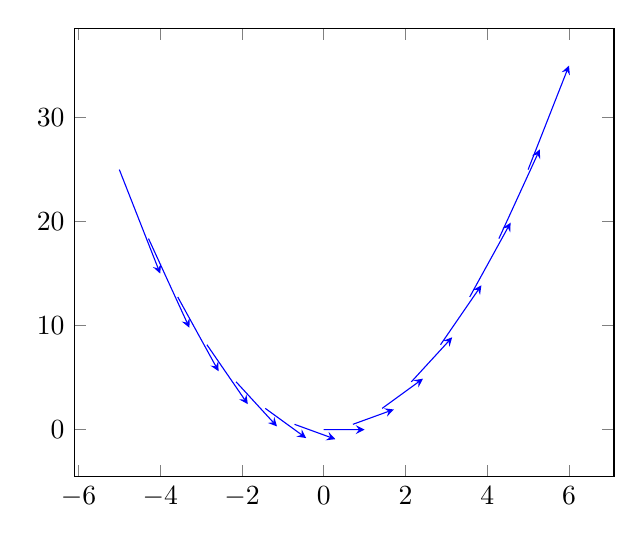
\begin{tikzpicture}
\begin{axis}
    \addplot [
        blue,
        quiver={u=1,v=2*x},
        -stealth,
        samples=15,
    ] {x^2};
\end{axis}
\end{tikzpicture}
\end{codeexample}

    基点 $(x,y)$ 像以前一样提供；在上例中，它由 |\addplot expression|
    生成并产生 $(x,x^2)$。此外还需要给出向量方向 $(u,v)$。我们的示例
    使用 |quiver/u=1| 和 |quiver/v=2*x|，得到 $u=1$ 和 $v=2x$。
    因此，我们为 $f(x) = x^2$ 的导数定义并可视化了一个向量场。

    一个常见的示例是可视化二维函数 $f(x,y)$ 的梯度
    $(\partial_x f,\partial_y f)(x,y)$：
    %
\pgfplotsexpensiveexample
\begin{codeexample}[]
\begin{tikzpicture}
\begin{axis}[
    title={$x \exp(-x^2-y^2)$ and its gradient},
    domain=-2:2,
    view={0}{90},
    axis background/.style={fill=white},
]
    \addplot3 [
        contour lua={number=9,labels=false},thick,
            ] {exp(0-x^2-y^2)*x};
    \addplot3 [
        blue,-stealth,samples=15,
        quiver={
            u={exp(0-x^2-y^2)*(1-2*x^2)},
            v={exp(0-x^2-y^2)*(-2*x*y)},
            scale arrows=0.3,
        },
    ] {exp(0-x^2-y^2)*x};
\end{axis}
\end{tikzpicture}
\end{codeexample}
    %
    \noindent 该示例首先使用 |contour gnuplot| 来可视化
    $f(x,y) = x\exp(-x^2-y^2)$。选项 |contour/number| 和
    |contour/labels| 用于对等高线进行微调，这里不涉及（|axis background|
    也是如此，它只是提高了等高线的可见性）。我们感兴趣的是 |quiver=|
    样式：它将 |u| 和 |v| 定义为某些二维表达式。此外，我们使用了
    |quiver/scale arrows| 来减小箭头大小。|-stealth| 是一个 \Tikz{}
    样式，用于配置 `|stealth|' 类型的外向箭头样式。|samples=15| 键
    配置了我们如何获取输入数据。在本例中，我们有输入数据
    $(x_i,y_j,f(x_i,y_j))$，其中 $i$ 和 $j$ 各有 $15$ 个采样。

    也可以将矢量图放置在指定的 $z$ 值上：
    %
\pgfplotsexpensiveexample
\begin{codeexample}[]
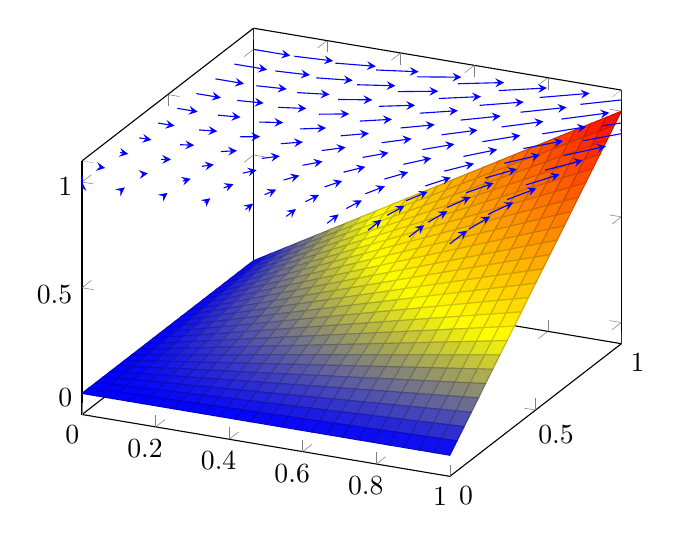
\begin{tikzpicture}
\begin{axis}[
    domain=0:1,
    xmax=1,
    ymax=1,
]
    \addplot3 [surf] {x*y};
    \addplot3 [
        blue,-stealth,samples=10,
        quiver,quiver/.cd,
            u=y,v=x,w=0,
            scale arrows=0.1,
    ] {1};
\end{axis}
\end{tikzpicture}
\end{codeexample}
    %
    \noindent 这里，矢量图放置在 |surf| 之上。它可视化梯度（使用公共
    比例因子 $1/10$ 来减小箭头长度）。|quiver/w=0| 表示箭头没有 $z$
    方向的差异，而 |{1}| 参数表示所有箭头从 $(x_i,y_j,1)$ 开始。
    这里，值 $(x_i,y_j)$ 在 |domain=0:1| 参数中采样（使用
    |samples=10|），即箭头从 $(x_i,y_j,1)$ 开始，到
    $(x_i+y_j/10, y_j+x_i/10, 1)$ 结束。

    到目前为止，矢量图不假设输入点的特殊顺序。这有两个后果：首先，
    你可以通过仅考虑 $(x,y) + (u,v)$（或 $(x,y,z) + (u,v,w)$）来绘制
    任何向量场——数据不一定需要是二维函数（不像 |surf| 等）。另一方面，
    你需要手动提供 |quiver/scale arrows|，因为当你提供矩阵数据时，
    |quiver| 不知道网格宽度\footnote{实际上，我将来可能会添加类似
    \texttt{quiver/scale arrows=auto} 的功能，我还不确定。在 \TeX{} 中
    遍历输入数据很慢，自动计算网格宽度更慢\ldots}。

    注意，矢量图目前不能与对数坐标轴一起使用。

    \begin{pgfplotskeylist}{%
        quiver/u=\meta{expression} (initially 0),
        quiver/v=\meta{expression} (initially 0),
        quiver/w=\meta{expression} (initially 0)%
    }
        这些键定义了向量方向 $(u,v)$（或者对于三维图，$(u,v,w)$）应如何
        设置。

        \meta{expression} 可以是像 |quiver/u=1| 或 |quiver/u=42*5|
        这样的常量表达式。它也可以取决于最终基点的值，如上例中使用
        |x|、|y| 或 |z| 值。在此上下文中，|x| 给出向量起始点的
        $x$ 坐标，|y| 给出 $y$ 坐标，依此类推。


        \paragraph{注意：}

        |x| 指的是\emph{最终的 $x$ 坐标}这一事实意味着参数图
        \emph{应使用 $t$ 作为变量}\footnote{抱歉造成这个可用性问题。}。
        考虑以下示例：
        %
\begin{codeexample}[]
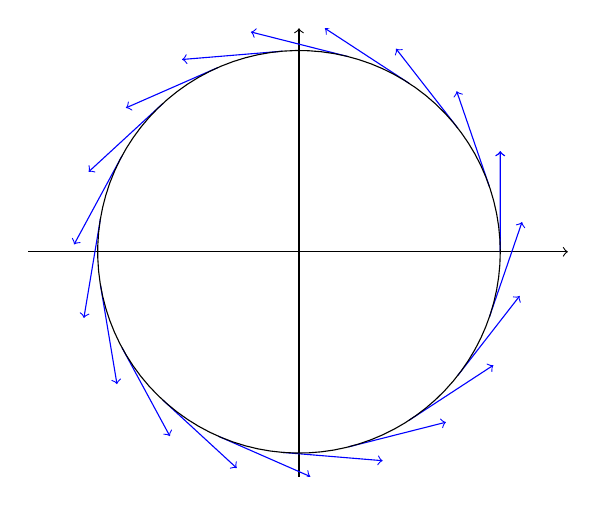
\begin{tikzpicture}
\begin{axis}[
    axis equal,
    axis lines=middle,
    axis line style={->},
    tick style={color=black},
    xtick=\empty,ytick=\empty,
]
    \addplot [samples=20, domain=0:2*pi,->,blue,
        % the default choice 'variable=\x' leads to
        % unexpected results here!
        variable=\t,
        quiver={
            u={-sin(deg(t))},
            v={cos(deg(t))},
            scale arrows=0.5,
        },
    ] ( {cos(deg(t))}, {sin(deg(t))} );
    \addplot [
        samples=100, domain=0:2*pi,
    ] ( {cos(deg(x))}, {sin(deg(x))} );
\end{axis}
\end{tikzpicture}
\end{codeexample}
        %
        \noindent 这里，使用参数图绘制一个圆和切向量。|variable=\t|
        的选择除了命名约定外还具有功能作用：它允许在 |u| 和 |v|
        的表达式中访问参数变量。另一方面，我们本可以使用 |u=y| 和
        |v=-x|，因为 |x| 展开为 $x$ 坐标，值为 |sin(deg(t))|，而 |y|
        展开为 $y$ 坐标 |cos(deg(t))|。

        另一个重要应用是将\emph{表列引用}（如 |quiver/u=\thisrow{col}|）
        与 |\addplot table| 结合使用：
        %
\begin{codeexample}[]
\begin{tikzpicture}
\begin{axis}[title=Quiver and plot table]
    \addplot [
        blue,
        quiver={u=\thisrow{u},v=\thisrow{v}},
        -stealth,
    ] table {
        x y u v
        0 0 1 0
        1 1 1 1
        2 4 1 4
        3 9 1 6
        4 16 1 8
    };
\end{axis}
\end{tikzpicture}
\end{codeexample}
        %
        \noindent 这里，\meta{expression} 使用了 |\thisrow|，它总是
        指 |\addplot table| 的实际行。

        注意，\meta{expression} 应始终为数值类型（目前不支持符号输入
        扩展）。
    \end{pgfplotskeylist}

    \begin{pgfplotskeylist}{%
        quiver/u value=\marg{value} (initially 0),
        quiver/v value=\marg{value} (initially 0),
        quiver/w value=\marg{value} (initially 0)%
    }
        这些键与 |quiver/u| 及其变体具有\emph{相同的功能}。但是，它们
        不调用数学解析器，因此只允许单值（包括类似 |\thisrow{columnname}|
        的内容）。
    \end{pgfplotskeylist}

    \begin{pgfplotskeylist}{%
        quiver/colored,
        quiver/colored=\marg{color}%
    }
        允许为每个箭头定义单独的颜色。省略参数 `\meta{color}' 等同于
        |quiver/colored=mapped color|，它使用 |point meta| 为每个箭头
        获取颜色。

        如果你只想为每个箭头设置相同的颜色，优先使用
        |\addplot[blue,quiver]|，它更高效。
    \end{pgfplotskeylist}

    \begin{pgfplotskey}{quiver/scale arrows=\marg{scale} (initially 1)}
        允许按因子重新缩放箭头。如果箭头长度大于相邻基点
        $(x_i,y_i)$ 之间的距离，这可能是必要的。将来可能会有自动
        重新缩放的功能。
    \end{pgfplotskey}

    \begin{pgfplotskey}{quiver/update limits=\mchoice{true,false} (initially true)}
        一个布尔值，指示点 $(x,y) + (u,v)$ 是否应贡献于坐标轴范围。
    \end{pgfplotskey}

    \begin{stylekey}{/pgfplots/quiver/every arrow (initially empty)}
        允许提供单独的箭头样式。

        该样式可以包含任何 \Tikz{} 绘图选项。它会为每个单独的箭头
        进行评估，并且可以取决于可视化时可用的任何内容。

        特别地，这包括 |point meta| 数据，通常使用
        |\pgfplotspointmetatransformed| $\in [0,1000]$，其中~$0$
        对应于 |point meta min|，~$1000$ 对应于 |point meta max|：
        %
    \label{pgfplots:example:pointmeta:quiver}
\begin{codeexample}[]
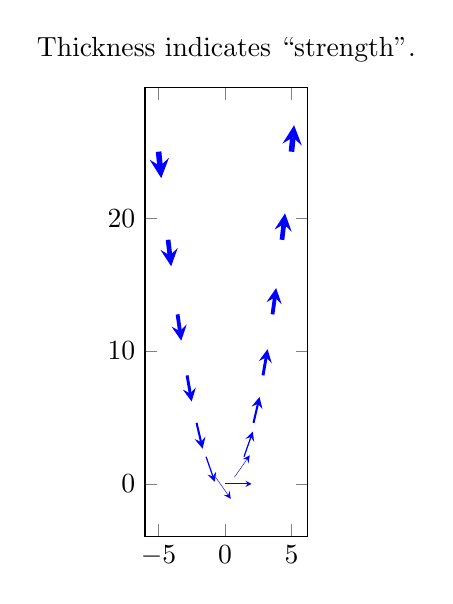
\begin{tikzpicture}
% define some constants:
\def\U{1}
\def\V{2*x}
\def\LEN{(sqrt((\U)^2 + (\V)^2)}

\begin{axis}[axis equal image,
    title=Thickness indicates ``strength''.
]
\addplot [blue,
  point meta={\LEN},
  quiver={
   u={(\U)/\LEN}, v={(\V)/\LEN},
   scale arrows=2,
   every arrow/.append style={
    line width=2pt*\pgfplotspointmetatransformed/1000
   },
  },
  -stealth,samples=15,
] {x^2};
\end{axis}
\end{tikzpicture}
\end{codeexample}
        %
        \noindent 在该示例中，我们将某个二维向量场存储在辅助常量
        |\U| 和 |\V| 中。每个向量的长度存储在 |\LEN| 中。|quiver|
        绘图本身包含单位长度向量——而 |\LEN| 进入 |every arrow|
        样式以获得不同的 |line width|。

        |every arrow| 样式也可以取决于 |mapped color|（前提是已设置
        |point meta|）。

        同样，如果你不需要单独的箭头样式，优先使用绘图样式
        （|cycle list| 或 |\addplot| 的参数），它更高效。
    \end{stylekey}

    \begin{pgfplotsxycodekeylist}{
        quiver/before arrow,
        quiver/after arrow%
    }
        用于更精细调整显示的高级键。它们允许在绘制单个箭头之前或
        之后手动安装一些 \TeX{} 代码。两者初始均为空。
    \end{pgfplotsxycodekeylist}

    \begin{stylekey}{/pgfplots/quiver/quiver legend}
        一个重新定义 |legend image code| 的样式，以便为 |quiver|
        图生成合适的图例。

        每当选择 |quiver| plot handler 时，它会被隐式激活。
        %
\begin{codeexample}[]
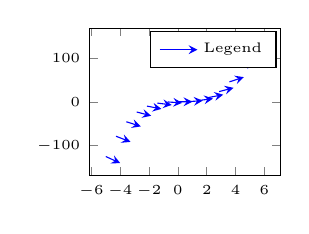
\begin{tikzpicture}
\begin{axis}[tiny]
    \addplot [
        blue,
        quiver={u=1,v=3*x},
        -stealth,
        samples=15,
    ] {x^3};
        \addlegendentry{Legend}
\end{axis}
\end{tikzpicture}
\end{codeexample}
    \end{stylekey}
\end{plottype}


\subsection{堆叠图}

\begin{pgfplotskey}{stack plots=\mchoice{x,y,false} (initially false)}
    允许沿 $x$ 或 $y$ 方向堆叠绘图。堆叠意味着将连续 |\addplot|
    命令的 $x$ 或 $y$ 坐标叠加在一起。
    %
\begin{codeexample}[]
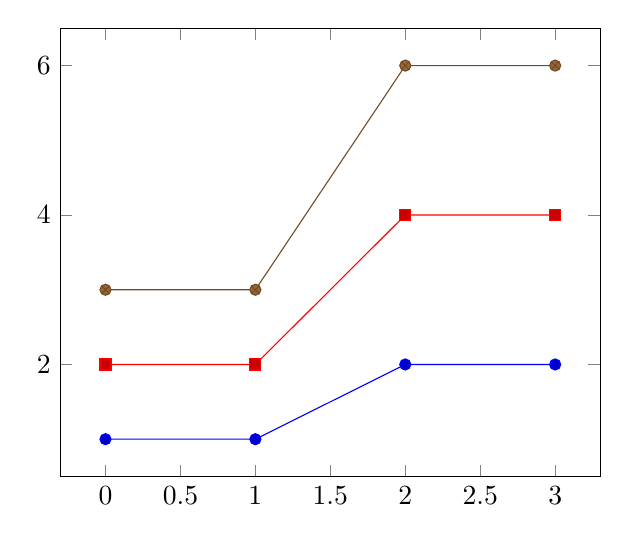
\begin{tikzpicture}
\begin{axis}[stack plots=y]
    \addplot coordinates {
        (0,1) (1,1) (2,2) (3,2)
    };
    \addplot coordinates {
        (0,1) (1,1) (2,2) (3,2)
    };
    \addplot coordinates {
        (0,1) (1,1) (2,2) (3,2)
    };
\end{axis}
\end{tikzpicture}
\end{codeexample}
    %
    当前 |stack plots| 的实现\emph{不会}插值缺失的坐标。这意味着如果
    绘图具有不同的网格，堆叠将失败。
\end{pgfplotskey}

\begin{stylekey}{/pgfplots/ybar stacked=\mchoice{plus,minus} (default plus)}
    plot handler |stack plots| 对柱状图特别有用。有两种可能的操作模式：
    第一种是设置 |stack plots=y,/tikz/ybar|。它仅激活这两个功能，
    而不让它们相互感知。第二种是设置 |ybar stacked|，它激活这两个
    功能\emph{并且}让它们相互感知。

    如果你将 |stack plots| 与 |/tikz/ybar| 一起使用，你会得到一种
    底层实现，有点"原始"：

\begin{codeexample}[]
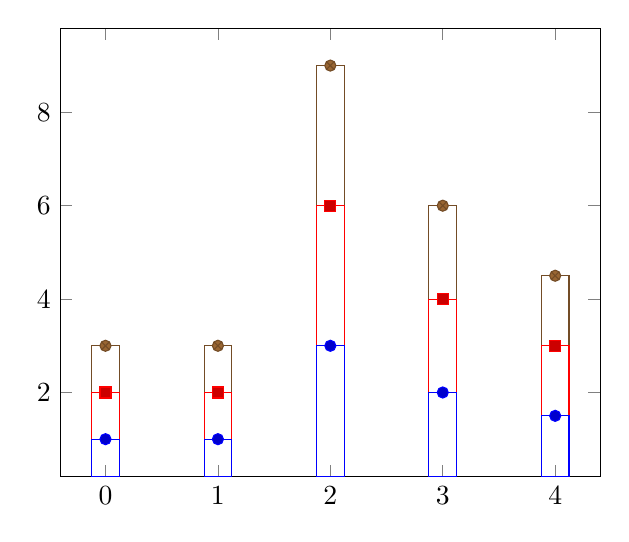
\begin{tikzpicture}
\begin{axis}[stack plots=y,/tikz/ybar]
    \addplot coordinates {
        (0,1) (1,1) (2,3) (3,2) (4,1.5)
    };
    \addplot coordinates {
        (0,1) (1,1) (2,3) (3,2) (4,1.5)
    };
    \addplot coordinates {
        (0,1) (1,1) (2,3) (3,2) (4,1.5)
    };
\end{axis}
\end{tikzpicture}
\end{codeexample}

    使用 |ybar stacked| 可启用堆叠垂直柱（即 |ybar| 和
    |stack plots=y|），\emph{并且}它还会调整图例和刻度外观，并分配
    一个有用的 |cycle list|。为此，它应作为选项提供给坐标轴：
    %
\begin{codeexample}[]
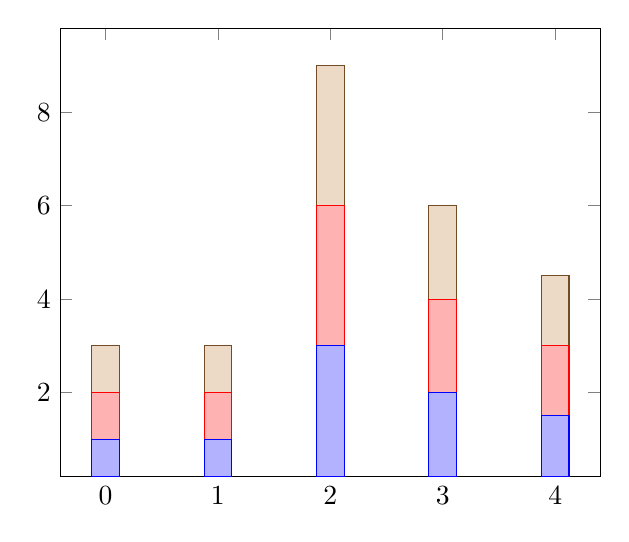
\begin{tikzpicture}
\begin{axis}[ybar stacked]
    \addplot coordinates {
        (0,1) (1,1) (2,3) (3,2) (4,1.5)
    };
    \addplot coordinates {
        (0,1) (1,1) (2,3) (3,2) (4,1.5)
    };
    \addplot coordinates {
        (0,1) (1,1) (2,3) (3,2) (4,1.5)
    };
\end{axis}
\end{tikzpicture}
\end{codeexample}

\begin{codeexample}[]
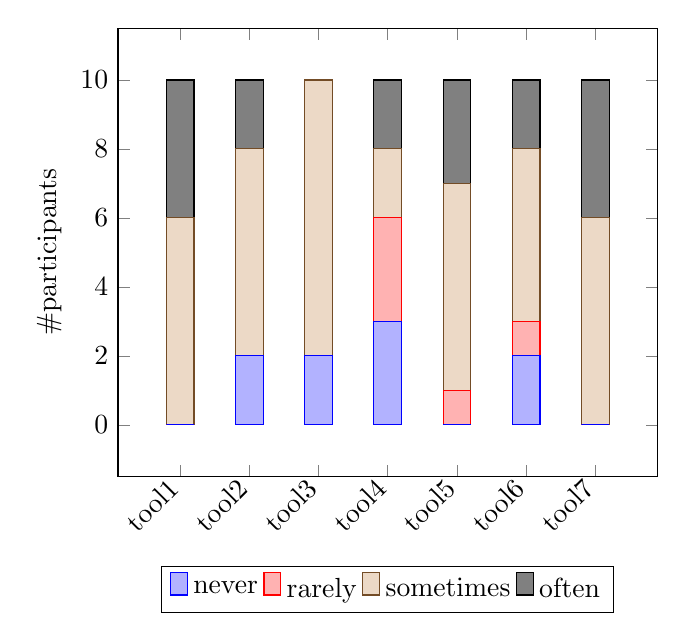
\begin{tikzpicture}
\begin{axis}[
    ybar stacked,
    enlargelimits=0.15,
    legend style={at={(0.5,-0.20)},
        anchor=north,legend columns=-1},
    ylabel={\#participants},
    symbolic x coords={tool1, tool2, tool3, tool4,
        tool5, tool6, tool7},
    xtick=data,
    x tick label style={rotate=45,anchor=east},
]
\addplot+ [ybar] coordinates {(tool1,0) (tool2,2)
  (tool3,2) (tool4,3) (tool5,0) (tool6,2) (tool7,0)};
\addplot+ [ybar] coordinates {(tool1,0) (tool2,0)
  (tool3,0) (tool4,3) (tool5,1) (tool6,1) (tool7,0)};
\addplot+ [ybar] coordinates {(tool1,6) (tool2,6)
  (tool3,8) (tool4,2) (tool5,6) (tool6,5) (tool7,6)};
\addplot+ [ybar] coordinates {(tool1,4) (tool2,2)
  (tool3,0) (tool4,2) (tool5,3) (tool6,2) (tool7,4)};
\legend{never, rarely, sometimes, often}
\end{axis}
\end{tikzpicture}
\end{codeexample}
\end{stylekey}

\begin{stylekey}{/pgfplots/xbar stacked=\mchoice{plus,minus} (default plus)}
    与 |ybar stacked| 相同的说明同样适用于 |xbar stacked|：
    |xbar stacked| 是一种整图范围内的样式，用于启用堆叠的水平柱状图
    （即\@ |xbar| 和 |stack plots=x|）。它还会调整图例和刻度
    外观，并分配一个有用的 |cycle list|。

    因此，可以有一幅结合了堆叠和柱状图的 ``原始'' 图片，
    如下面这幅图所示（即\@ 不使用 |xbar stacked|）：
    %
\begin{codeexample}[]
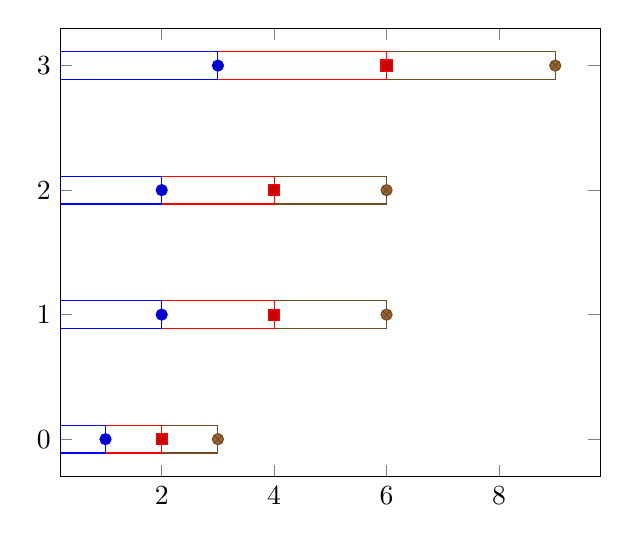
\begin{tikzpicture}
\begin{axis}[stack plots=x,/tikz/xbar]
    \addplot coordinates {
        (1,0) (2,1) (2,2) (3,3)
    };
    \addplot coordinates {
        (1,0) (2,1) (2,2) (3,3)
    };
    \addplot coordinates {
        (1,0) (2,1) (2,2) (3,3)
    };
\end{axis}
\end{tikzpicture}
\end{codeexample}

    或者，也可以在 |\begin{axis}| 之后直接激活 |xbar stacked|，
    并受益于多种样式调整。
    %
\begin{codeexample}[]
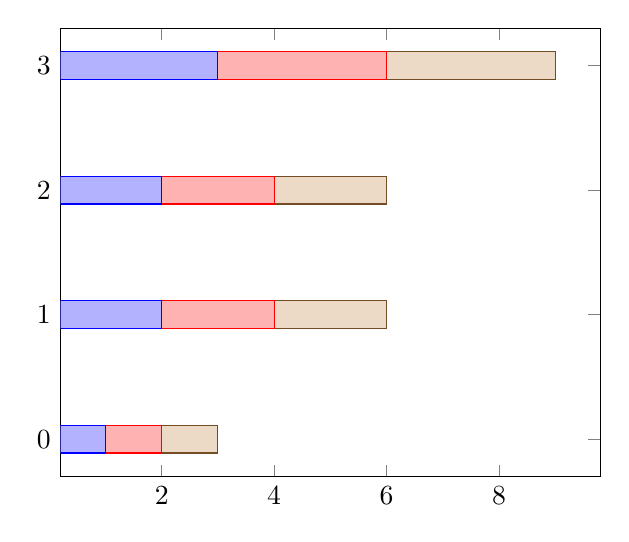
\begin{tikzpicture}
\begin{axis}[xbar stacked]
    \addplot coordinates {
        (1,0) (2,1) (2,2) (3,3)
    };
    \addplot coordinates {
        (1,0) (2,1) (2,2) (3,3)
    };
    \addplot coordinates {
        (1,0) (2,1) (2,2) (3,3)
    };
\end{axis}
\end{tikzpicture}
\end{codeexample}
\end{stylekey}

\begin{pgfplotskey}{stack dir=\mchoice{plus,minus} (initially plus)}
    配置 |stack plots| 的方向。值 |plus| 将连续绘图的坐标相加，而
    |minus| 将它们相减。
\end{pgfplotskey}

\begin{pgfplotskey}{reverse stacked plots=\mchoice{true,false} (initially true, default true)}
    配置堆叠绘图的绘制顺序。这或多或少是一个技术细节，在任何正常
    情况下都不应更改。

    其动机如下：假设有多个 |\addplot| 命令彼此堆叠，并且按出现顺序
    处理。那么，第二个绘图可能很容易将其线（或填充区域）绘制在第一个
    之上——完全隐藏其标记或线。因此，\PGFPlots{} 会反转绘制命令的顺序。

    这有一个副作用：坐标轴内任何正常的 \Tikz{} 路径也会按相反顺序
    处理。
\end{pgfplotskey}

\begin{pgfplotskey}{stacked ignores zero=\mchoice{true,false} (initially true, default true)}
    配置堆叠图以忽略"零"增量。

    在此上下文中，"忽略"意味着如果增量为零则抑制可视化。

    配置 |\pgfplotsset{compat=1.9}|（或更高版本）会为 |xbar stacked|
    和 |ybar stacked| 激活此功能。

    \begin{pgfplotskeylist}{%
        stacked ignores zero/default=\mchoice{true,false} (initially true),
        stacked ignores zero/markers=\mchoice{true,false} (initially true),
        stacked ignores zero/errorbars=\mchoice{true,false} (initially false)%
    }
        一个细节键，允许自定义如何以及在何处应用
        |stacked ignores zero|。除非
        |stacked ignores zero=true|，
        否则此键\emph{被忽略}。其默认配置是为标准可视化和标记抑制
        空增量的可视化。不过，误差棒仍会显示（即使增量为 $0$，误差棒
        通常也是非空的）。
    \end{pgfplotskeylist}
\end{pgfplotskey}

\begin{stylekey}{/pgfplots/xbar interval stacked=\mchoice{plus,minus} (default plus)}
    一个类似于 |/pgfplots/xbar stacked| 的样式，用于基于间隔的柱状图
    变体。
\end{stylekey}

\begin{stylekey}{/pgfplots/ybar interval stacked=\mchoice{plus,minus} (default plus)}
    一个类似于 |/pgfplots/ybar stacked| 的样式，用于基于间隔的柱状图
    变体。
\end{stylekey}


\subsubsection{堆叠柱状图与节点坐标}

可以将 |ybar stacked| 和 |xbar stacked| 与 |nodes near coords|
结合使用。与非堆叠图不同，在堆栈顶部附近绘制节点的用途似乎有限。
相反，人们通常希望看到每个堆叠步骤中添加的\emph{差值}。为此，
\PGFPlots{} 会自动重新配置 |nodes near coords|，以在每个新柱的
中心显示添加的值：

\begin{codeexample}[]
% needs \pgfplotsset{compat=1.9} or newer!
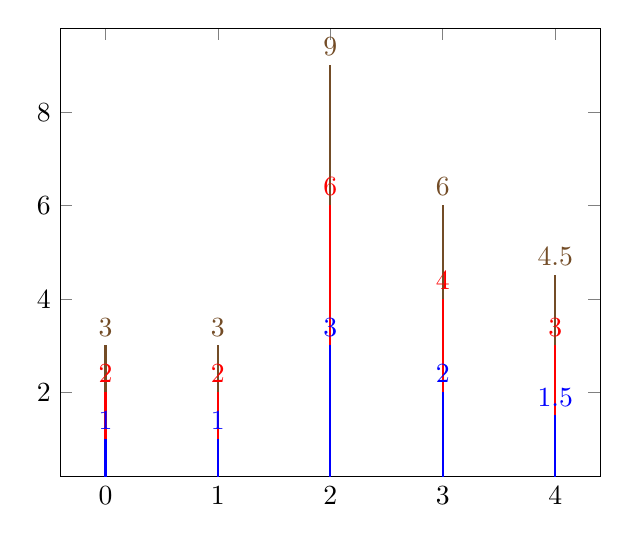
\begin{tikzpicture}
\begin{axis}[
    ybar stacked,nodes near coords,
    bar width=0.4,
]
    \addplot coordinates
        {(0,1) (1,1) (2,3) (3,2) (4,1.5)};
    \addplot coordinates
        {(0,1) (1,1) (2,3) (3,2) (4,1.5)};
    \addplot coordinates
        {(0,1) (1,1) (2,3) (3,2) (4,1.5)};
\end{axis}
\end{tikzpicture}
\end{codeexample}

\begin{codeexample}[]
% needs \pgfplotsset{compat=1.9} or newer!
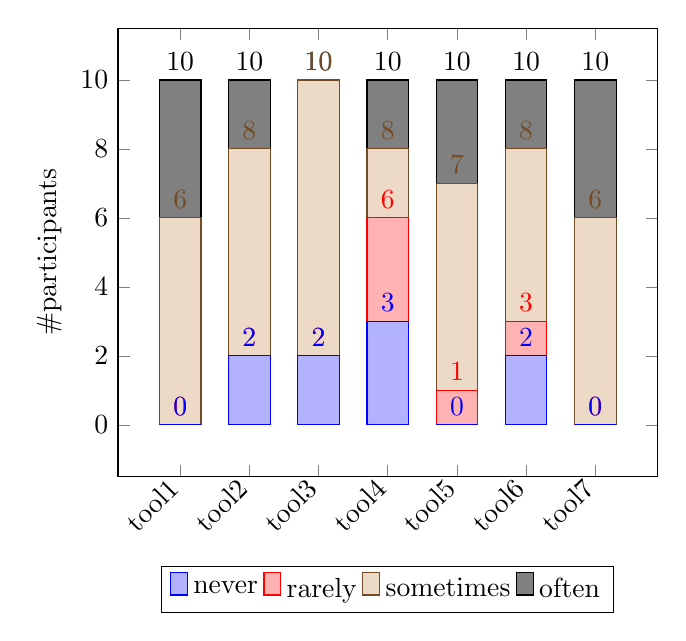
\begin{tikzpicture}
\begin{axis}[
    ybar stacked,
    bar width=15pt,
    nodes near coords,
    enlargelimits=0.15,
    legend style={at={(0.5,-0.20)},
        anchor=north,legend columns=-1},
    ylabel={\#participants},
    symbolic x coords={tool1, tool2, tool3, tool4,
        tool5, tool6, tool7},
    xtick=data,
    x tick label style={rotate=45,anchor=east},
]
\addplot+ [ybar] coordinates {(tool1,0) (tool2,2)
  (tool3,2) (tool4,3) (tool5,0) (tool6,2) (tool7,0)};
\addplot+ [ybar] coordinates {(tool1,0) (tool2,0)
  (tool3,0) (tool4,3) (tool5,1) (tool6,1) (tool7,0)};
\addplot+ [ybar] coordinates {(tool1,6) (tool2,6)
  (tool3,8) (tool4,2) (tool5,6) (tool6,5) (tool7,6)};
\addplot+ [ybar] coordinates {(tool1,4) (tool2,2)
  (tool3,0) (tool4,2) (tool5,3) (tool6,2) (tool7,4)};
\legend{never, rarely, sometimes, often}
\end{axis}
\end{tikzpicture}
\end{codeexample}

注意，前面的示例不包含值为~|0| 的坐标的节点。这是由于键
|stacked ignores zero|，当 |compat=1.9| 或更新版本时它是激活的：
空增量将被丢弃。

这种自动重新配置本质上是样式 |xbar stacked| 或 |ybar stacked|
的一部分：两者都会重新配置 |nodes near coords|。注意，此功能是在
1.9 版本中引入的。为了保持与以前变通方法的向后兼容性，你必须写入
|compat=1.9| 才能获得这些效果。

\begin{codeexample}[]
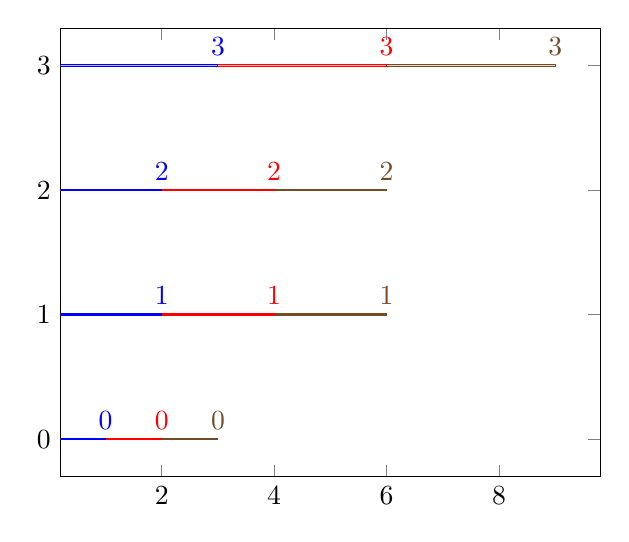
\begin{tikzpicture}
\begin{axis}[
    xbar stacked,nodes near coords,
    bar width=0.5,
]
    \addplot coordinates
        {(1,0) (2,1) (2,2) (3,3)};
    \addplot coordinates
        {(1,0) (2,1) (2,2) (3,3)};
    \addplot coordinates
        {(1,0) (2,1) (2,2) (3,3)};
\end{axis}
\end{tikzpicture}
\end{codeexample}


\subsubsection{带负值的堆叠图}

|xbar stacked| 或 |ybar stacked| 中负值的含义及其可视化取决于用例，
需要明确定义。\PGFPlots{} 在堆叠图的上下文中提供了两种不同的负值
解释：

\begin{pgfplotskey}{stack negative=\mchoice{on previous,separate} (initially separate)}
    选项 \declaretext{on previous} 会简单地将输入数据中找到的任何值
    相加。因此，如果你有四个彼此堆叠的图，第一个值为 $10$，第二个值
    $50$，第三个值 $-10$，第四个值 $30$，则最终值将为
    $10+50-10+30 = 80$。然而，将负尺寸的柱可视化为通常的
    |xbar stacked| 图很难阅读，并且在此上下文中需要垂直偏移。
    可以如下实现：
    %
\begin{codeexample}[]
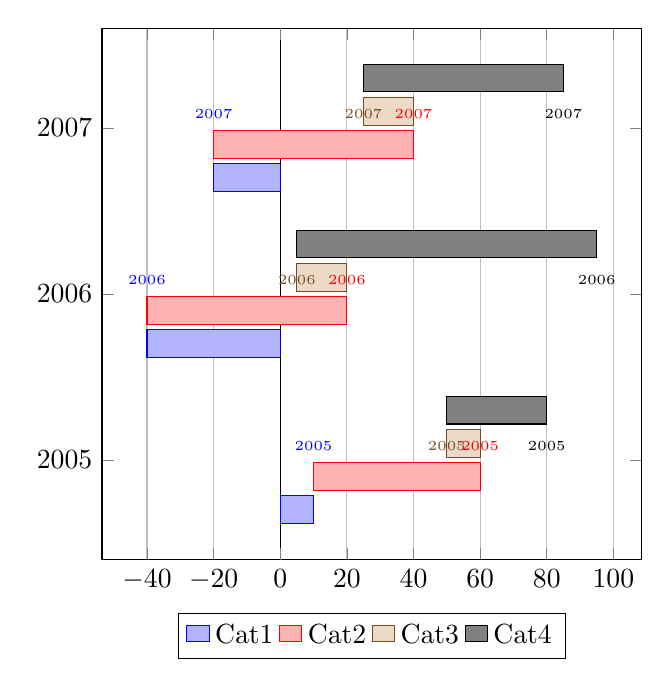
\begin{tikzpicture}
    \pgfplotstableread{
        Year  Cat1  Cat2  Cat3  Cat4
        2005  10    50    -10   30
        2006  -40   60    -15   90
        2007  -20   60    -15   60
    }\mytable
\begin{axis}[
    xbar stacked,
    stack negative=on previous,
    %
    xmajorgrids,
    legend style={at={(0.5,-0.1)},
        anchor=north,legend columns=-1},
    bar width=10pt,
    bar shift auto,
    nodes near coords,
    nodes near coords style={font=\tiny},
    y=60pt,
    ytick distance=1,
    enlarge y limits=0.3,
    /pgf/number format/1000 sep=,
    extra x ticks={0},
    extra x tick style={grid style={black},
    xticklabel=\empty},
]
    \addplot table [x index=1,y=Year] {\mytable};
    \addplot table [x index=2,y=Year] {\mytable};
    \addplot table [x index=3,y=Year] {\mytable};
    \addplot table [x index=4,y=Year] {\mytable};
    \legend{Cat1,Cat2,Cat3,Cat4}
\end{axis}
\end{tikzpicture}
\end{codeexample}

    在这种情况下，$y=2005$ 的值类似于我们的输入案例
    $10+50-10+30=80$。这是一个"普通"的 |xbar stacked|，配置为
    |stack negative=on previous|——但使用了特殊键 |bar shift auto|，
    它也用于创建分组的 |xbar| 图：每个 |\addplot| 都获得一个垂直偏移。

    尽管与"瀑布图"\index{waterfall chart}相似，但这并不打算成为瀑布图。
    在撰写本文时，\PGFPlots{} 不支持瀑布图。

    选项 |stack negative=on previous| 是以下情况的\emph{初始}值
    %
    \begin{itemize}
        \item 除堆叠柱状图外的所有图，
        \item 如果 |compat| 小于 |1.13| 则为所有图。
    \end{itemize}
    %
    从 |compat=1.13| 开始，|stack negative| 的初始值对于
    |xbar stacked|、|ybar stacked| 及其基于 |* interval| 的变体为
    |separate|。

    另一个选项 \declaretext{separate} 对负值和非负值\emph{分别}跟踪
    柱的起点：
    %
\begin{codeexample}[]
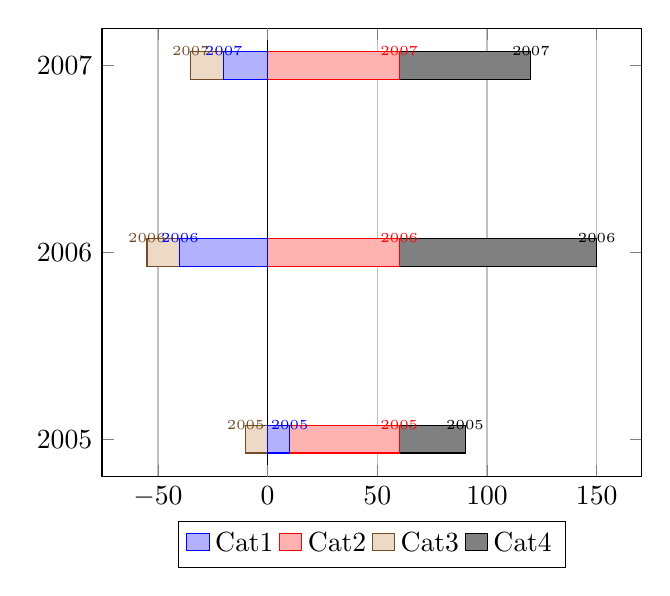
\begin{tikzpicture}
    \pgfplotstableread{
        Year  Cat1  Cat2  Cat3  Cat4
        2005  10    50    -10   30
        2006  -40   60    -15   90
        2007  -20   60    -15   60
    }\mytable
\begin{axis}[
    xbar stacked,
    % is default anyway:
    stack negative=separate,
    %
    /pgf/number format/1000 sep=,
    xmajorgrids,
    nodes near coords,
    nodes near coords style={font=\tiny},
    ytick distance=1,
    legend style={at={(0.5,-0.1)},
        anchor=north,legend columns=-1},
    extra x ticks={0},
    extra x tick style={grid style={black},
    xticklabel=\empty},
]
    \addplot table [x index=1,y=Year] {\mytable};
    \addplot table [x index=2,y=Year] {\mytable};
    \addplot table [x index=3,y=Year] {\mytable};
    \addplot table [x index=4,y=Year] {\mytable};
    \legend{Cat1,Cat2,Cat3,Cat4}
\end{axis}
\end{tikzpicture}
\end{codeexample}

    在这种情况下，正贡献延伸到正 $x$ 轴，而负贡献延伸到负 $x$ 轴。
    没有最终总和（或者更好地说：有两个最终总和）。其效果就像你定义了
    两个单独的坐标轴，一个用于正贡献，一个用于负贡献，并在原点对齐。

    从 |compat=1.13| 开始，|stack negative=separate| 是堆叠柱状图的
    初始设置。较旧的兼容级别使用 |stack negative=on previous|。
\end{pgfplotskey}


\subsection{面积图}

面积图指的是在几条曲线之间填充区域的二维图。注意，这是一个相当不完整
的描述，因为 |mesh|、|surf|ace 和 |patch| 图当然也是某种"面积图"。

本节涵盖两种类型的面积图，即由 |stack plots| 定义的那些和使用
|\addplot fill between| 定义的那些。


\subsubsection{使用堆叠图填充}

填充绘图之间区域的第一个（也是较旧的）选项是 |\closedcycle| 和
|stack plots| 的组合。它们可以与任何其他图类型结合使用。

\begin{codeexample}[]
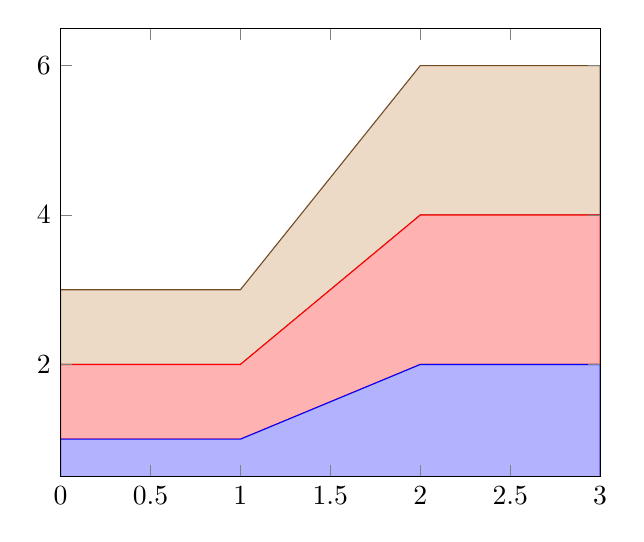
\begin{tikzpicture}
\begin{axis}[
    stack plots=y,
    area style,
    enlarge x limits=false,
]
    \addplot coordinates
        {(0,1) (1,1) (2,2) (3,2)}
            \closedcycle;
    \addplot coordinates
        {(0,1) (1,1) (2,2) (3,2)}
            \closedcycle;
    \addplot coordinates
        {(0,1) (1,1) (2,2) (3,2)}
            \closedcycle;
    \end{axis}
\end{tikzpicture}
\end{codeexample}
%
\noindent 这种面积可视化的主要特性是，坐标轴的所有绘图被放在一起，
并且由于它们是堆叠的，因此形成了区域。

\noindent 面积图可能需要修改图例，例如使用 |area legend| 键。此外，
可能需要考虑 |axis on top| 键，以使填充区域不会重叠刻度和网格线，
因为此类图通常覆盖坐标轴的大部分区域。

注意，依赖于 |stack plots| 的面积图有一个严重限制：当且仅当每个图
具有相同的坐标时（在我们 |stack plots=y| 的案例中，每个图具有相同的
$x$ 坐标），堆叠才能工作。

\begin{stylekey}{/pgfplots/area style}
    一个设置以下内容的样式
    %
\begin{codeexample}[code only]
\pgfplotsset{
    /pgfplots/area style/.style={
        area cycle list,
        area legend,
        axis on top,
    },
}
\end{codeexample}
\end{stylekey}

\begin{stylekey}{/pgfplots/area cycle list}
    一种安装适用于面积图的 |cycle list| 的样式。此样式的初始
    配置只是调用 |bar cycle list|，该列表
    也提供了填充的绘图样式。
\end{stylekey}

\begin{codeexample}[]
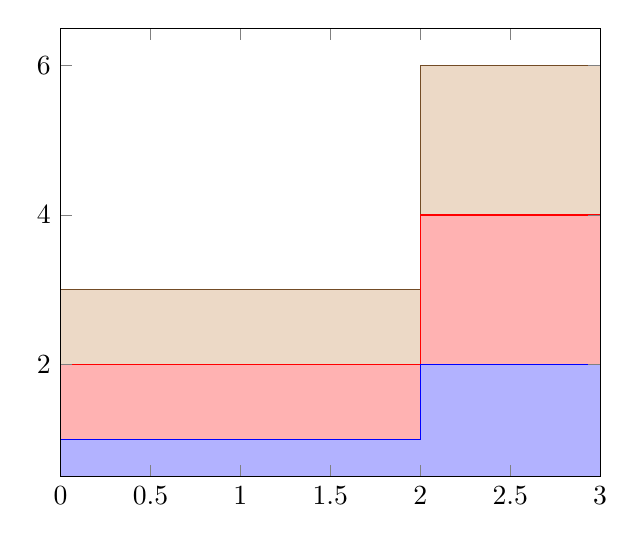
\begin{tikzpicture}
    \begin{axis}[
        const plot,
        stack plots=y,
        area style,
        enlarge x limits=false,
    ]
    \addplot coordinates
        {(0,1) (1,1) (2,2) (3,2)}
            \closedcycle;
    \addplot coordinates
        {(0,1) (1,1) (2,2) (3,2)}
            \closedcycle;
    \addplot coordinates
        {(0,1) (1,1) (2,2) (3,2)}
            \closedcycle;
    \end{axis}
\end{tikzpicture}
\end{codeexample}

\begin{codeexample}[]
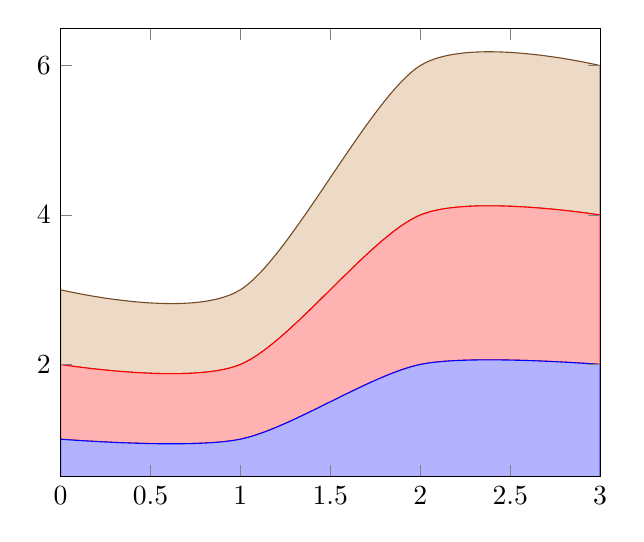
\begin{tikzpicture}
    \begin{axis}[
        smooth,
        stack plots=y,
        area style,
        enlarge x limits=false,
    ]
    \addplot coordinates
        {(0,1) (1,1) (2,2) (3,2)}
            \closedcycle;
    \addplot coordinates
        {(0,1) (1,1) (2,2) (3,2)}
            \closedcycle;
    \addplot coordinates
        {(0,1) (1,1) (2,2) (3,2)}
            \closedcycle;
    \end{axis}
\end{tikzpicture}
\end{codeexample}

\begin{codeexample}[]
\pgfplotstableread{pgfplots.timeseries.dat}\loadedtable
\pgfplotstabletypeset\loadedtable
\end{codeexample}

\begin{codeexample}[]
    \pgfplotstableread{pgfplots.timeseries.dat}{\loadedtable}
\begin{tikzpicture}
    \begin{axis}[
        ymin=0,
        minor tick num=4,
        enlarge x limits=false,
        axis on top,
        every axis plot post/.append style={mark=none},
        const plot,
        legend style={
            area legend,
            at={(0.5,-0.15)},
            anchor=north,
            legend columns=-1,
        },
    ]
        \addplot [draw=blue,fill=blue!30!white]
            table [x=time,y=1minload]       from \loadedtable
                \closedcycle;
        \addplot table [x=time,y=nodes]     from \loadedtable;
        \addplot table [x=time,y=cpus]      from \loadedtable;
        \addplot table [x=time,y=processes] from \loadedtable;
        \legend{1min load,nodes,cpus,processes}
    \end{axis}
\end{tikzpicture}
\end{codeexample}

\begin{codeexample}[width=4cm]
    \pgfplotstableread{pgfplots.timeseries.dat}\loadedtable
\begin{tikzpicture}
    \begin{axis}[
        ymin=0,
        minor tick num=4,
        enlarge x limits=false,
        const plot,
        axis on top,
        stack plots=y,
        cycle list={
            {blue!70!black,fill=blue},
            {blue!60!white,fill=blue!30!white},
            {draw=none,fill={rgb:red,138;green,82;blue,232}},
            {red,thick}
        },
        ylabel={Mem [GB]},
        legend style={
            area legend,
            at={(0.5,-0.15)},
            anchor=north,
            legend columns=2},
    ]
    \addplot  table [x=time,y=memused]      from \loadedtable \closedcycle;
    \addplot  table [x=time,y=memcached]    from \loadedtable \closedcycle;
    \addplot  table [x=time,y=membuf]       from \loadedtable \closedcycle;
    \addplot+ [stack plots=false]
              table [x=time,y=memtotal]     from \loadedtable;
    \legend{Memory used,Memory cached,Memory buffered,Total memory}
    \end{axis}
\end{tikzpicture}
\end{codeexample}


\subsubsection{在命名的绘图下方/之间填充}
\label{sec:fillbetween:in:area:plots}

{%
\pgfkeys{
    /pgfmanual/gray key prefixes/.add={}{,/tikz/fill between/},
    /pdflinks/search key prefixes in/.add={}{,/tikz/fill between/},
}

填充绘图下方或之间区域的第二种方式是 \PGFPlots{} 附带的 |fillbetween|
库。

\tikzname{} 允许使用 |name path| 为绘图或路径命名。|fillbetween|
库提供了特殊的"图类型" |\addplot fill between|，它期望输入两个这样的
命名路径。然后，它在这些命名路径之间生成填充区域。

与上一节讨论的通过 |stack plots| 实现的面积图相比，最大的不同在于
|\addplot fill between| 接受\emph{任意}输入图：坐标可以不同，范围可以
不同，甚至可以组合 |smooth| 和 |sharp plot|。此外，|\addplot fill between|
允许通过其 |soft clip| 功能仅选择两个输入路径之间的子区域，并且它接受
使用其样式 |every even segment|、|every segment no| \meta{index}
等单独设置样式的填充段。

参考文档在 \ref{sec:fillbetween} 节，但以下示例试图涵盖"填充之间"
的基本用例。请参阅 \ref{sec:fillbetween} 节的参考文档，以深入讨论
每个涉及的键。

以下高级示例使用 |soft clip| 选择两个部分区域以填充这些区域：
%
\begin{codeexample}[]
% requires \usepgfplotslibrary{fillbetween}
\begin{tikzpicture}
\begin{axis}
    \addplot+ [name path=A,domain=0:5] {x^2};

    \path [name path=B]
        (\pgfkeysvalueof{/pgfplots/xmin},0) --
        (\pgfkeysvalueof{/pgfplots/xmax},0);

    \addplot [gray] fill between [
        of=A and B,soft clip={domain=3:4},
    ];
    \addplot [gray!30] fill between [
        of=A and B,soft clip={domain=2:3},
    ];
\end{axis}
\end{tikzpicture}
\end{codeexample}

前面的示例以两条路径为特征，每条路径都使用 |name path| 命名。名为
`|A|' 的路径是 $x^2$ 的图。另一条名为 `|B|' 的路径实际上就是可见的
$x$ 轴，|\path| 指令意味着它根本不会被绘制。注意，
|\pgfkeysvalueof{/pgfplots/xmin}| 展开为可见的下 $x$ 轴范围。最后，
我们看到两条 |\addplot fill between| 指令，都带有选择
|of=A and B|，并且都带有（不同的）|soft clip| 值。|soft clip| 键将
填充段限制为由某条路径 \meta{lower corner}| rectangle |\meta{upper corner}
定义的边界矩形，其中两个参数是不可见矩形包围盒的下角和上角。在我们的
案例中，该包围盒由某些 |domain| 限制以及上下坐标轴范围定义。只有
填充段的那些部分构成 |\addplot fill between| 的结果。

当描边涉及的路径 `|A|' 或 `|B|' 时，这种对特定间隔（或更好地说：矩形）
的限制也可用：\PGFPlots{} 附带了 |decoration=soft clip|，它可以与
|postaction| 组合，如下所示。
%
\begin{codeexample}[]
% requires \usepgfplotslibrary{fillbetween}
\begin{tikzpicture}
\begin{axis}
    % define some common macro
    \def\clippath{
        (3,-1) rectangle (4,100)
    }
    \draw [help lines] \clippath;

    \addplot+ [name path=A,domain=0:5,
        mark=none,
        postaction={decorate,red,line width=2pt,
            decoration={
                soft clip,
                soft clip path={\clippath},
            },
        },
    ] {x^2};

    \path [name path=B]
        (\pgfkeysvalueof{/pgfplots/xmin},0) --
        (\pgfkeysvalueof{/pgfplots/xmax},0);

    \addplot [orange] fill between [
        of=A and B,soft clip={\clippath},
    ];
\end{axis}
\end{tikzpicture}
\end{codeexample}
%
前面的示例有一个 |\def\clippath|，它定义了一个可重用的包围盒。这里，
|fill between| 语句与前面的示例类似，唯一的区别是我们的宏被用作值。
主要区别在于图 `|A|' 中的 |postaction|。|postaction| 是一个 \tikzname{}
构造，允许两次绘制同一路径。第二次绘制图时使用 |postaction| 之后的
选项列表。在我们的案例中，它是一个 |decoration|，将以 |red| 和粗线
绘制。|decoration| 应用了一个 |soft clip| 路径。在此上下文中，
|soft clip| 仅应用于一条路径，但思想是相同的：仅显示 |soft clip|
参数内的部分。

注意，|fill between| 也可以用于任意图，而不仅仅是 $x$ 轴。实际上，
可以组合任意两个图。
%
\begin{codeexample}[]
% requires \usepgfplotslibrary{fillbetween}
\begin{tikzpicture}
\begin{axis}
    \addplot [blue,name path=A,domain=0:5] {x^2};
    \addplot [red,name path=B,smooth] table {
        x y
        0 10
        1 8
        2 6
        3 1
        4 5
    };
    \addplot [gray!50] fill between [
        of=A and B,
        soft clip={domain=3:4},
    ];
    \addplot [gray!10,draw=black] fill between [
        of=A and B,
        soft clip={domain=1:2.5},
    ];
\end{axis}
\end{tikzpicture}
\end{codeexample}
%
\noindent 前面的示例有两个图，采样数量不同、范围不同、输入方法也不同。
尽管如此，这两个图之间的区域仍然可以像前面的示例一样填充，包括任何
交点。

也可以为填充段定义单独的样式。为此，必须设置 |split| 键，它会激活
单独的输出路径。这使得可以使用特殊样式，如下例所示。这里，我们有两个
带有显式编号段索引的样式：
%
\begin{codeexample}[]
% requires \usepgfplotslibrary{fillbetween}
\begin{tikzpicture}
\begin{axis}
    \addplot [blue,name path=A,domain=0:5] {x^2};
    \addplot [red,name path=B,smooth] table {
        x y
        0 10
        1 8
        2 6
        3 1
        4 5
    };
    \addplot [gray] fill between [
        of=A and B,
        split,
        every segment no 0/.style=
            {pattern color=gray!50,
             pattern=north east lines},
        every segment no 1/.style=
            {pattern=north west lines},
    ];
\end{axis}
\end{tikzpicture}
\end{codeexample}
%
\noindent 注意，该示例没有 |soft clip| 参数。因此，它在涉及路径的起点
和终点之间填充。|split| 参数与样式结合产生单独绘制的填充段。

延伸阅读：参见 \ref{sec:fillbetween} 节。
}


\subsection{闭合绘图（填充绘图下方的区域）}
\label{sec:pgfplots:closingplots}

\begin{command}{\closedcycle}
    在 |\addplot| 之后将 |\closedcycle| 作为 \meta{尾部路径命令} 使用，
    可从最后一个绘图坐标到第一个坐标绘制一条闭合线。

    当你希望填充绘图下方的区域时，请使用 |\closedcycle|。

\begin{codeexample}[]
\begin{tikzpicture}
\begin{axis}
    \addplot {x^2+2} \closedcycle;
\end{axis}
\end{tikzpicture}
\end{codeexample}

\begin{codeexample}[]
\begin{tikzpicture}
\begin{axis}
    \addplot+ [fill] {x^2+2} \closedcycle;
\end{axis}
\end{tikzpicture}
\end{codeexample}
    %
    对于堆叠图，|\closedcycle| 会将当前绘图与上一个绘图连接起来，
    而不是与 $x$ 轴连接。\footnote{堆叠图的实现需要一些额外的逻辑来
    确定填充区域：\lstinline{\\closedcycle} 会生成一个
    \texttt{plot coordinates} 命令，其中使用了上一个绘图的\emph{反向}
    坐标。这对最终用户通常无关紧要，但它假设绘图类型是对称的。
    由于阶梯图本质上是非对称的，\lstinline{\\closedcycle} 会将
    \texttt{const plot mark right} 用作 \texttt{const plot mark left}
    的反向序列。}
    %
\begin{codeexample}[]
\begin{tikzpicture}
\begin{axis}[stack plots=y]
    \addplot+ [fill] coordinates {
        (0,1) (1,1) (2,2) (3,2)
    }
        \closedcycle
    ;
    \addplot+ [fill] coordinates {
        (0,1) (1,1) (2,2) (3,2)
    }
        \closedcycle
    ;
\end{axis}
\end{tikzpicture}
\end{codeexample}
\end{command}

闭合绘图同样适用于\emph{三维坐标轴}，详见第\pageref{sec:pgfplots:filled:line}页的\ref{sec:pgfplots:filled:line}节。

注意，|\closedcycle| 是为函数设计的（即每个 $x$ 至多对应一个 $y$
值的绘图）。对于任意曲线，你可以放心地使用 \tikzname{} 路径
\declareandlabel{--cycle}，它只是简单地连接最后一个路径元素和第一个：
%
\begin{codeexample}[]
\begin{tikzpicture}
\begin{axis}
    \addplot coordinates {
        (0,1) (1,2) (0,3) (-1,2)
    };
\end{axis}
\end{tikzpicture}
\end{codeexample}

\begin{codeexample}[]
\begin{tikzpicture}
\begin{axis}
    \addplot coordinates {
        (0,1) (1,2) (0,3) (-1,2)
    }
        --cycle
    ;
\end{axis}
\end{tikzpicture}
\end{codeexample}

\begin{codeexample}[]
\begin{tikzpicture}
\begin{axis}
    \addplot+ [fill] coordinates {
        (0,1) (1,2) (0,3) (-1,2)
    }
        --cycle
    ;
\end{axis}
\end{tikzpicture}
\end{codeexample}

实际上，|--cycle| 是 \cite{tikz} 的一条路径指令；它连接一条路径的
第一个和最后一个坐标。注意，对于 |fill| 填充的路径，这一操作会自动完成。



\subsection{散点图}
\label{sec:pgfplots:scatter:2d}

最简单的散点图产生与上面线图相同的结果——但它们仅包含标记。使用
\Tikz{} 的 |only marks| 键来启用它们。

\begin{plottype}{only marks}
    绘制一个简单的散点图：所有标记具有相同的外观。
    %
\begin{codeexample}[]
\begin{tikzpicture}
\begin{axis}[enlargelimits=false]
    \addplot+ [
        only marks,
        samples=400,
    ] {rand};
\end{axis}
\end{tikzpicture}
\end{codeexample}
    %
    |only marks| 可视化样式简单地在每个坐标处绘制标记。标记可以用
    |mark=|\meta{mark name} 设置，标记选项（如大小和颜色）可以使用
    |mark options=|\meta{style options} 键指定（或通过修改 |every mark|
    样式）。可用的标记以及可接受的样式选项可以在第\pageref{sec:markers}页的
    \ref{sec:markers} 节中找到。
\end{plottype}

    \label{pgfplots:scatter}
更复杂的散点图会为每个数据点改变标记外观。一个例子是标记颜色取决于
函数值 $f(x)$ 的大小或其他提供的坐标。在以下各节中，术语"散点图"
将用于这种类型的图。

散点图需要"源"坐标。这些源坐标可以是 $y$ 坐标，或显式提供的额外值。

\begin{plottype}[/pgfplots]{scatter}
    启用标记外观修改。默认实现为每个数据点获取"源"坐标（参见下文的
    |scatter src|），并将它们线性映射到当前颜色图中。所得颜色用作
    标记的绘制和填充颜色。

\begin{codeexample}[]
\begin{tikzpicture}
\begin{axis}
    \addplot+ [
        scatter,
        only marks,
        samples=50,
        scatter src=y,
    ] {x - x^2};
\end{axis}
\end{tikzpicture}
\end{codeexample}

    键 |scatter| 只是一个布尔变量，用于启用标记修改。它仅适用于标记，
    并且可以与任何其他图类型组合。

\begin{codeexample}[]
\begin{tikzpicture}
\begin{axis}
    \addplot+ [
        scatter,
        samples=50,
        scatter src=y,
    ] {x^3};
\end{axis}
\end{tikzpicture}
\end{codeexample}
\end{plottype}

散点图可以使用一组选项进行配置。其中一个选项是
必选的，其余选项允许对标记外观选项进行精细控制。

\begin{pgfplotskey}{scatter src=\mchoice{%
        none,
        \meta{expression},
        x,y,z,
        f(x),
        explicit,
        explicit symbolic%
    } (initially none)%
}
\label{pgfplots:scatter:src}
    此键对于任何散点图都是必需的，并且一旦激活 |scatter| 且未做出
    不同选择，它就会被设置为 |f(x)|。它需要作为 |\addplot| 的
    \meta{option} 提供，以配置用于确定标记外观的值。实际上，
    |scatter src| 不过是 |point meta| 的别名，因此此键的主要文档在
    第\pageref{pgfplots:pointmeta}页。不过，我们在这里将选择项与
    散点图示例一起总结。

    通常，|scatter src| 提供输入数据（数值或字符串类型），用于确定
    标记的颜色和其他样式选项。默认配置期望数值数据，该数据被线性映射
    到当前颜色图中。

    |scatter src| 的值决定如何获取此数据：选项 \declaretext{x}、
    \declaretext{y} 和 \declaretext{z} 将分别使用 $x$、$y$ 或 $z$
    坐标来确定标记选项。任何坐标过滤器、对数或堆叠图计算都已应用于
    这些值（对未处理的值使用 |rawx|、|rawy| 和 |rawz|）。特殊选项
    |f(x)| 对于二维图等同于 |y|，对于三维图等同于 |z|。选项
    \declaretext{explicit} 期望散点源数据作为来自坐标输入流的额外
    坐标（关于如何提供输入元数据，参见 \ref{sec:pgfplots:providing:input}
    节，或参见下文的一些小示例）。它们将被视为数值数据。选项
    \declaretext{explicit symbolic} 也期望散点源数据作为每个输入坐标的
    额外元信息，但它将它们视为字符串而非数值数据。因此，不执行任何
    算术运算。散点图样式的任务是对其进行处理。例如，参见下文的
    |scatter/classes| 样式。最后，可以提供任意数学表达式，它涉及零个、
    一个或多个值 \declaretext{x}（当前 $x$ 坐标）、\declaretext{y}
    （当前 $y$ 坐标）或 \declaretext{z}（当前 $z$ 坐标，如果有）。

    如果从表中读取数据，数学表达式还可能涉及 |\thisrow|\marg{column name}
    或 |\thisrowno|\marg{column index}，以访问当前行中的任何表单元格。

    以下是如何为选项 \declaretext{explicit} 和 \declaretext{explicit
    symbolic} 提供数据的示例。
    %
\begin{codeexample}[code only]
\begin{tikzpicture}
    \begin{axis}
        % provide color data explicitly using [<data>]
        % behind coordinates:
        \addplot+ [scatter,scatter src=explicit]
            coordinates {
                (0,0) [1.0e10]
                (1,2) [1.1e10]
                (2,3) [1.2e10]
                (3,4) [1.3e10]
                % ...
            };

        % Assumes a datafile.dat like
        % xcolname  ycolname    colordata
        % 0         0           0.001
        % 1         2           0.3
        % 2         2.1         0.4
        % 3         3           0.5
        % ...
        % the file may have more columns.
        \addplot+ [scatter,scatter src=explicit]
            table [x=xcolname,y=ycolname,meta=colordata]
                {datafile.dat};
        % Same data as last example:
        \addplot+ [scatter,scatter src=\thisrow{colordata}+\thisrow{ycolname}]
            table [x=xcolname,y=ycolname]
                {datafile.dat};

        % Assumes a datafile.dat like
        % 0         0           0.001
        % 1         2           0.3
        % 2         2.1         0.4
        % 3         3           0.5
        % ...
        % the first three columns will be used here:
        \addplot+ [scatter,scatter src=explicit]
            file {datafile.dat};
    \end{axis}
\end{tikzpicture}
\end{codeexample}

    请注意，|scatter src|$\neq$|none| 即使在 |scatter=false| 时也会
    产生计算工作。
\end{pgfplotskey}

\begin{stylekey}{/pgfplots/scatter/use mapped color=\marg{options for each marker}
    (initially draw=mapped color!80!black,fill=mapped color)%
}
    此样式默认安装。激活时，它通过将 |scatter src| 坐标线性转换到
    当前颜色图中，为每个处理的点坐标重新计算颜色 |mapped color|。
    然后，它评估作为 \meta{options for each marker} 提供的选项，
    这些选项预期取决于 |mapped color|。

    颜色图的用户界面在 \ref{sec:pgfplots:colormap} 节中描述。

\begin{codeexample}[]
\begin{tikzpicture}
\begin{axis}[title=Default arguments]
    \addplot+ [
        scatter,
        scatter src=y,
    ] {2*x+3};
\end{axis}
\end{tikzpicture}
\end{codeexample}

\begin{codeexample}[]
\begin{tikzpicture}
\begin{axis}[
    title=Black fill color and varying draw color,
    scatter/use mapped color={
        draw=mapped color,
        fill=black,
    },
]
    \addplot+ [
        scatter,
        scatter src=y,
    ] {2*x+3};
\end{axis}
\end{tikzpicture}
\end{codeexample}

\begin{codeexample}[]
\begin{tikzpicture}
\begin{axis}[
    title=Black draw color and varying fill color,
    scatter/use mapped color={
        draw=black,
        fill=mapped color,
    },
]
    \addplot+ [
        scatter,
        scatter src=y,
    ] {2*x+3};
\end{axis}
\end{tikzpicture}
\end{codeexample}

\message{Expecting '/pgfplots/warning/approx empty range enlarged' here.^^J}%
\begin{codeexample}[]
\begin{tikzpicture}
    \begin{axis}[colormap/bluered,colorbar]
    \addplot3+ [
        samples=4,
        z buffer=sort,
        % enable scatter:
        scatter,
        % redefine appearance:
        scatter/use mapped color={ball color=mapped color},
        % configure input:
        scatter src=rand,
        only marks,
        mark=ball,
        mark size=3pt,
    ] {0};
    \end{axis}
\end{tikzpicture}
\end{codeexample}
    %
    此键实际上是一个样式，它重新定义了 |@pre marker code| 和
    |@post marker code|（见下文）。


    \paragraph{备注：}

    样式 |use mapped color| \emph{重}定义了 |@pre marker code| 和
    |@post marker code|。有一个带星号的变体
    \declareandlabel{use mapped color*}，它\emph{追加}功能，同时保留
    旧的标记代码。
\end{stylekey}

\begin{stylekey}{/pgfplots/scatter/classes=\marg{styles for each class name}}
\label{pgfplots:scatterclasses}
    一种散点图样式，使用多个类别来可视化点。该样式假设每个点坐标都附有一个类别标签，即假设使用选项 |scatter src=explicit symbolic|。\footnote{如果 \texttt{scatter src} 不是
    \texttt{explicit symbolic}，我们期望一个数值参数，该参数四舍五入
    到最近的整数。所得整数用作类别标签。如果失败，则将数值参数截断
    到最近的整数。如果也失败，则该点没有标签。} 类别标签可以是数字，
    但也可以是符号常量。给定每个点的类别标签，
    \meta{styles for each class name} 包含一个逗号分隔的列表，该列表
    将外观选项与每个类别标签关联。

\begin{codeexample}[]
\begin{tikzpicture}
\begin{axis}[
    scatter/classes={
        a={mark=square*,blue},
        b={mark=triangle*,red},
        c={mark=o,draw=black}   % <-- don't add comma
    },
]
    % \addplot[] is better than \addplot+[] here:
    % it avoids scalings of the cycle list
    \addplot [
        scatter,only marks,
        scatter src=explicit symbolic,
    ] coordinates {
        (0.1,0.15)  [a]
        (0.45,0.27) [c]
        (0.02,0.17) [a]
        (0.06,0.1)  [a]
        (0.9,0.5)   [b]
        (0.5,0.3)   [c]
        (0.85,0.52) [b]
        (0.12,0.05) [a]
        (0.73,0.45) [b]
        (0.53,0.25) [c]
        (0.76,0.5)  [b]
        (0.55,0.32) [c]
    };
\end{axis}
\end{tikzpicture}
\end{codeexample}
    %
    在这个示例中，坐标 |(0.1,0.15)| 具有关联标签 `|a|'，而
    |(0.45,0.27)| 具有标签 `|c|'（关于指定点元数据的详情，参见
    \ref{sec:addplot} 节）。现在，|scatter/classes| 的参数包含每个
    标签的样式——对于标签 `|a|'，将以蓝色绘制方形标记。

    图例的生成与普通图一样——但 |scatter/classes| 为每个提供的类别
    要求一个图例条目。它自动将类别标签传达给图例。其工作方式就像
    有不同的 |\addplot| 命令，每个类别标签一个。

    也可以将 |scatter/classes| 作为单个绘图的参数提供，从而在一个
    坐标轴中允许不同的散点图。
    %
\begin{codeexample}[]
\begin{tikzpicture}
\begin{axis}[legend pos=south east]
    % The data file contains:
    % x     y      label
    % 0.1   0.15   a
    % 0.45  0.27   c
    % 0.02  0.17   a
    % 0.06  0.1    a
    % 0.9   0.5    b
    % 0.5   0.3    c
    % 0.85  0.52   b
    % 0.12  0.05   a
    % 0.73  0.45   b
    % 0.53  0.25   c
    % 0.76  0.5    b
    % 0.55  0.32   c
    \addplot [
        % clickable coords={\thisrow{label}},
        scatter/classes={
            a={mark=square*,blue},
            b={mark=triangle*,red},
            c={mark=o,draw=black,fill=black}% no comma
        },
        scatter,only marks,
        scatter src=explicit symbolic,
    ] table [x=x,y=y,meta=label]
        {plotdata/scattercl.dat};

    \addplot coordinates
        {(0.1,0.1) (0.5,0.3) (0.85,0.5)};
    \legend{Class 1,Class 2,Class 3,Line}
\end{axis}
\end{tikzpicture}
\end{codeexample}

    一般来说，\meta{styles for each class name} 的格式是
    \meta{label}|=|\marg{style options} 的逗号分隔列表。


    \paragraph{注意：}

    键 |every mark| 和 |mark options| 在 \meta{styles for each class
    name} 内部使用时\emph{无效}！因此，你不必分配 |mark options|，
    可以直接提供选项。反正它们仅适用于标记。


    \paragraph{备注：}

    要将 |\label| 和 |\ref| 与 |scatter/classes| 结合使用，可以将类别
    标签作为可选参数以方括号形式提供给 |\label|：

\begin{codeexample}[code only]
\addplot [
    scatter/classes={
        a={mark=square*,blue},
        b={mark=triangle*,red},
        c={mark=o,draw=black,fill=black}    % <-- don't add comma here
    },
    scatter,only marks,
    scatter src=explicit symbolic,
]
    % [and coordinate input here... ]
;

\label[a]{label:for:first:class}
\label[b]{label:for:second:class}
\label[c]{label:for:third:class}

...
First class is \ref{label:for:first:class}, second is \ref{label:for:second:class}.
\end{codeexample}


    \paragraph{备注：}

    可以点击图中以显示带鼠标弹出窗口的标签，参见 |clickable| 库的
    |clickable coords| 键。

    \paragraph{备注：}

    样式 |scatter/classes| \emph{重}定义了 |@pre marker code| 和
    |@post marker code|。有一个带星号的变体
    \declareandlabel{scatter/classes*}，它\emph{追加}功能，同时保留
    旧的标记代码。
\end{stylekey}

\begin{pgfplotskeylist}{%
    nodes near coords=\marg{content} (default \textbackslash pgfmathprintnumber\textbackslash pgfplotspointmeta),
    nodes near coords*=\marg{content} (default \textbackslash pgfmathprintnumber\textbackslash pgfplotspointmeta)%
}
\labelprefix\label{pgfplots:example:pointmeta:nodesnearcoords}
    一种 |scatter| 图样式，在每个坐标附近放置文本节点。

\begin{codeexample}[]
\begin{tikzpicture}
\begin{axis}[nodes near coords]
    \addplot+ [
        only marks
    ] coordinates {
        (0.5,0.2) (0.2,0.1) (0.7,0.6)
        (0.35,0.4) (0.65,0.1)
    };
\end{axis}
\end{tikzpicture}
\end{codeexample}
    %
    如果没有指定其他内容，则 \meta{content} 就是
    ``point meta'' 的内容，使用默认方式显示：
    \meta{content}=|\pgfmathprintnumber{\pgfplotspointmeta}|。宏
    |\pgfplotspointmeta| 包含由 |point meta| 键所选择的内容，
    对于二维图，它默认为 $y$-坐标，对于三维图
    默认为 $z$-坐标。

    由于 |point meta=explicit symbolic| 允许处理字符串数据，因此你可以
    提供文本描述，这些描述将显示在所生成的
    节点中：\footnote{在这种情况下，|\textbackslash pgfmathprintnumber| 将
    被自动跳过。}
    %
\begin{codeexample}[]
\begin{tikzpicture}
\begin{axis}[nodes near coords,enlargelimits=0.2]
    \addplot+ [
        only marks,
        point meta=explicit symbolic,
    ] coordinates {
        (0.5,0.2) [(1)]
        (0.2,0.1) [(2)]
        (0.7,0.6) [(3)]
        (0.35,0.4) [(4)]
        (0.65,0.1) [(5)]
    };
\end{axis}
\end{tikzpicture}
\end{codeexample}
    %
    方括号是为 |\addplot coordinates| 提供显式 |point meta| 的方式。
    关于如何从文件获取点元数据，请参阅 |plot file| 和 |\addplot table|
    的文档。

    \meta{content} 也可以取决于 |\pgfplotspointmeta| 以外的东西。但由于
    \meta{content} 在 |\end{axis}| 期间评估，\PGFPlots{} 可能不知道
    \meta{content} 内部的任何特殊信息——你需要按如下方式使用
    |visualization depends on| 键将其传达给 \PGFPlots{}：
    %
\begin{codeexample}[width=3cm]
\begin{tikzpicture}
    \begin{axis}[enlargelimits=0.2]
        \addplot [
            scatter,mark=*,only marks,
            % we use 'point meta' as color data...
            point meta=\thisrow{color},
            % ... therefore, we can't use it as argument for nodes near coords ...
            nodes near coords*={$(\pgfmathprintnumber[frac]\myvalue)$},
            % ... which requires to define a visualization dependency:
            visualization depends on={\thisrow{myvalue} \as \myvalue},
        ] table {
            x      y    color   myvalue
            0.5    0.2  1       0.25
            0.2    0.1  2       1.5
            0.7    0.6  3       0.75
            0.35   0.4  4       0.125
            0.65   0.1  5       2
        };
    \end{axis}
\end{tikzpicture}
\end{codeexample}
    %
    \noindent 该示例使用 |scatter| 图来获得不同的颜色，其中
    |scatter src|（或等价的 |point meta|）已用于定义标记颜色。除了
    彩色的 |scatter| 图之外，我们还想添加 |nodes near coords|，其中
    显示的节点应包含 |\thisrow{myvalue}|。为此，我们定义
    |scatter,point meta=\thisrow{color}|（如前几节所述）。此外，我们使用
    \declare{nodes near coords*} 来\emph{组合}不同的 |scatter| 样式
    （详情见下文）。|nodes near coords*| 的值取决于 |\thisrow{myvalue}|，
    但我们不能使用 |\pgfplotspointmeta|（它已被占用）。因此，我们通过
    |visualization depends on={\thisrow{myvalue} \as \myvalue}| 来传达
    额外的输入数据。该语句定义了一个新宏 |\myvalue|，并赋值
    |\thisrow{myvalue}|。此外，它配置 \PGFPlots{} 记住这个特定宏及其
    内容，直到 |\end{axis}|（详情参见 |visualization depends on| 的
    文档）。

    样式 |nodes near coords| 可能对柱状图有用，关于 |nodes near coords|
    的示例参见 |ybar|。


    \paragraph{备注与细节：}

    \begin{itemize}
        \item |nodes near coords| 对当前绘图的线样式和颜色使用相同的
            选项。可以使用样式 |every node near coord| 更改，见下文。
        \item |nodes near coords| 实际上是 |scatter| 图样式之一。它
            重新定义 |scatter/@pre marker code| 以生成几个 \Tikz{}
            |\node| 命令。

            为了将 |nodes near coords| 与其他 |scatter| 图样式（如
            |scatter/use mapped color| 或 |scatter/classes|）一起使用，
            你可以在每个键后附加一个星号。变体
            \declareandlabel{nodes near coords*} 将\emph{追加}代码到
            |scatter/@pre marker code|，而不覆盖先前的值。
        \item 如果文本被裁剪掉，考虑将 |enlargelimits| 与
            |nodes near coords| 一起使用。
        \item 目前 |nodes near coords| 对 |ybar interval| 或
            |xbar interval| 不能令人满意地工作，抱歉。
    \end{itemize}
\end{pgfplotskeylist}

\begin{stylekey}{/pgfplots/every node near coord}
    用于 |nodes near coords| 生成的每个节点的样式。它初始为空。
\end{stylekey}

\pgfplotsshortstylekey nodes near coords style=every node near coord\pgfeov
\pgfplotsshortstylekey node near coords style=every node near coord\pgfeov
\pgfplotsshortstylekey node near coord style=every node near coord\pgfeov

\begin{pgfplotskey}{nodes near coords align=\marg{alignment method} (initially auto)}
    指定如何对齐 |nodes near coords| 生成的节点。

    \meta{alignment method} 的可能选项有

    \begin{description}
        \item[]\declare{auto} 如果显示 $x$ 坐标则使用 |horizontal|，
            在所有其他情况下使用 |vertical|。这会检查 |point meta| 的
            当前值。
        \item[]\declare{horizontal} 如果 |\pgfplotspointmeta| $<0$
            则使用 |left|，否则使用 |right|。
        \item[]\declare{vertical} 如果 |\pgfplotspointmeta| $<0$
            则使用 |below|，否则使用 |above|。
        \item[] 也可以提供任何 \Tikz{} 对齐选项，如
            |anchor=north east|、|below| 或类似选项。也允许多个选项。
    \end{description}
\end{pgfplotskey}

\begin{pgfplotskeylist}{%
    coordinate style/.condition=\marg{expression}\marg{options},
    coordinate style/.from=\marg{something expanding to options},
    coordinate style/.clear%
}
\labelprefix\label{key:coordinatestyle}
    这些键允许为\emph{选定的}坐标定义 \meta{options}。

    第一个键 \declareandlabel{coordinate style/.condition} 接收一个
    \meta{expression}，并将其 \meta{options} 与所有匹配的坐标关联：
    %
\begin{codeexample}[]
\begin{tikzpicture}
\begin{axis}
    \addplot+ [
        nodes near coords,
        only marks,
        coordinate style/.condition=
            {\coordindex==0}{below},
        coordinate style/.condition=
            {\coordindex==1}{red},
        coordinate style/.condition=
            {x < 2.1 && y > 4}{green},
        point meta=explicit symbolic,
    ] table [meta=label] {
        Depth Breadth label
        2.57  3.59    Cambridge
        2.58  4.27    Dresden
        2.45  3.77    {Palo Alto}
        2.61  2.10    Asan
        2.03  4.17    Heidelberg
        2.25  4.29    Yamagata
    };
\end{axis}
\end{tikzpicture}
\end{codeexample}
    %
    该图使用 |\addplot table| 并将文本信息与每个数据点关联。此外，
    它使用三个 |coordinate style| 条件来修改这些点中几个的外观。
    因此，标签"Cambridge"放置在其坐标下方，"Dresden"以红色绘制，
    "Heidelberg"以绿色绘制。

    第二种可能性 \declareandlabel{coordinate style/.from} 是无条件的，
    从公共源定义样式信息。其主要用途是定义一个对每个点展开为不同值
    的源，例如使用 |\thisrow|：
    %
\begin{codeexample}[]
\begin{tikzpicture}
\begin{axis}
    \addplot+ [
        nodes near coords,
        only marks,
        coordinate style/.from=
            \thisrow{style},
        coordinate style/.condition=
            {x < 2.1 && y > 4}{black},
        point meta=explicit symbolic,
    ] table [meta=label] {
        Depth Breadth label       style
        2.57  3.59    Cambridge   below
        2.58  4.27    Dresden     red
        2.45  3.77    {Palo Alto} green
        2.61  2.10    Asan        {}
        2.03  4.17    Heidelberg  {left}
        2.25  4.29    Yamagata    {}
    };
\end{axis}
\end{tikzpicture}
\end{codeexample}
    %
    我们重用了上面的示例，但增加了第四列"style"，它成为
    |coordinate style/.from| 的一部分，并为每个单独的坐标分配
    \meta{options}。注意，"Heidelberg"也匹配第二个条件样式，因此它
    获得额外的选项 |left|（从"style"列读取）和 |black|（来自
    |coordinate style|）。注意，"Asan"和"Yamagata"在 style 列中具有
    空值，并以从绘图继承的正常样式绘制。

    最后，|coordinate style/.clear| 删除所有先前配置的值。

    所有 |coordinate style| 都是激活的。如果一个坐标匹配多个
    |coordinate style|，它将按照 |coordinate style| 定义在文件中出现的
    相同顺序接收所得选项。

    注意，|coordinate style| 会覆盖 |nodes near coords align|（而后者
    在 |coordinate style| 内不受支持）。

    键 |coordinate style| 也对其他图类型有用且可用。以下示例基于普通的
    |scatter| 图，其中红点接收特殊选项：
    %
\begin{codeexample}[]
\begin{tikzpicture}
\begin{axis}
    \addplot+ [
        scatter,
        coordinate style/.condition=
            {abs(x-1) < 0.001}{scale=3,xshift=4pt},
    ] coordinates {(0,0) (0.5,0.5) (1,1)};
\end{axis}
\end{tikzpicture}
\end{codeexample}
    %
    这里，我们使用公式 $\lvert x-1 \rvert < 0.001$ 来识别点坐标，并
    增大关联标记的大小并移动其位置。在此上下文中，使用考虑舍入问题
    的条件通常是一个好的做法，即避免使用等于运算符。

    在撰写本文时，|coordinate style| 受以下 plot handlers 支持：
    %
    \begin{itemize}
        \item |scatter|,
        \item |scatter explicit color|,
        \item |nodes near coords|,
        \item |scatter/classes|.
    \end{itemize}

    另见第\pageref{sec:coordinate:style}页的 \ref{sec:coordinate:style}
    节中的示例。
\end{pgfplotskeylist}

\begin{pgfplotskey}{scatter/position=\mchoice{absolute,relative} (initially relative)}
    允许选择如何定位散点图标记。这仅在 |scatter| 选项为 |true| 时
    适用。

    选项 \declaretext{relative} 是初始配置，它意味着散点标记放置在
    给定点的坐标处。从技术上讲，它意味着变换矩阵被平移，使得
    |(0,0)| 恰好在当前点的坐标处。这通常是你想要的。

    选项 \declaretext{absolute} 允许绝对定位散点图标记，例如通过
    |axis cs|。这可以与 |nodes near coords| 以及
    |every node near coord/.style=|\marg{options} 中合适的一组
    \meta{options} 组合：可以写类似
    |at={(\coordindex,\coordindex*5)}| 的东西。注意，此选项必须需要
    一个 |at| 键来指定节点的位置，否则其位置将是未定义的。
    \footnote{好吧，它将是画布的原点。这不一定与你的坐标轴原点相同。}
\end{pgfplotskey}

\begin{pgfplotsxycodekeylist}{%
    scatter/@pre marker code,
    scatter/@post marker code%
}
\labelprefix\label{pgfplots:example:pointmeta:scatter}
    这两个键构成了公共接口，它根据散点源坐标确定标记外观。

    重新定义它们允许对标记类型、线样式和颜色进行细粒度控制。

    散点图算法工作如下：
    %
    \begin{enumerate}
        \item 散点源坐标形成一个数据流，其数据范围除坐标轴范围外还
            会被计算。对于 |symbolic| 元数据，此步骤会被跳过。
        \item 在绘制任何标记之前，初始化从这些数据范围到区间
            $[0.0,1000.0]$ 的线性坐标变换。
        \item 每个散点源坐标\footnote{在评估期间，公共宏
            \texttt{\textbackslash pgfplotspointmeta} 和
            \texttt{\textbackslash pgfplotspointmetarange} 以 $a:b$
            的格式指示源坐标和源坐标范围（对于对数轴，它们以定点表示
            给出；对于线性轴，以浮点给出）。}将被线性变换，结果作为
            宏 |\pgfplotspointmetatransformed| $ \in [0.0,1000.0]$
            可用。

            因此，决策基于数据范围的千分比。对于 |symbolic| 元数据，
            变换会被跳过（元数据仅包含在上述宏中）。
        \item \pgfname{} 坐标系被平移，使得 |(0pt,0pt)| 是绘图坐标。
        \item 评估 |scatter/@pre marker code| 的代码（无参数）。
        \item 评估绘制标记的标准代码。
        \item 评估 |scatter/@post marker code| 的代码（无参数）。
    \end{enumerate}
    %
    其思想是生成一组取决于 |\pgfplotspointmetatransformed| 的外观键。
    然后，以 |@pre| 代码形式调用 |\scope|\oarg{generated keys} 以及
    以 |@post| 代码形式关联的 |\endscope|，将使用 \oarg{generated
    keys} 单独绘制标记。

    下面展示了一个技术示例。它演示了如何编写用户定义的例程，在此案例
    中是一个三类系统。\footnote{请注意，你不需要复制这个特定示例：
    多类示例也可以作为预定义样式 \texttt{scatter/classes} 使用。}
    %
\begin{codeexample}[]
\begin{tikzpicture}
% Low-Level scatter plot interface Example:
% use three different marker classes
% 0% -- 30%   : first class
% 30% -- 60%  : second class
% 60% -- 100% : third class
\begin{axis}[
  scatter/@pre marker code/.code={
    \ifdim\pgfplotspointmetatransformed pt<300pt
      \def\markopts{mark=square*,fill=blue}
    \else
      \ifdim\pgfplotspointmetatransformed pt<600pt
        \def\markopts{mark=triangle*,fill=orange}
      \else
         \def\markopts{mark=pentagon*,fill=red}
      \fi
    \fi
    \expandafter\scope\expandafter[\markopts]
  },
  scatter/@post marker code/.code={
    \endscope
  },
]
    \addplot+ [scatter,scatter src=y,samples=40]
       {sin(deg(x))};
\end{axis}
\end{tikzpicture}
\end{codeexample}
    %
    请注意，|\ifdim| 比较的是 \TeX{} 长度，因此该示例在此上下文中使用的
    任何数字都带有 |pt| 后缀。这不改变语义。两个（！）|\expandafter|
    构造确保 |\scope| 以 |\markopts| 的\emph{内容}而非宏名
    |\markopts| 被调用。
\end{pgfplotsxycodekeylist}


\subsection{一维彩色网格图}
\label{sec:1d:mesh}

\begin{plottype}[/pgfplots]{mesh}
    使用当前颜色图来确定每个固定线段的颜色。每个线段将获得相同的颜色。
    %
\begin{codeexample}[]
\begin{tikzpicture}
\begin{axis}
    \addplot [mesh] {x + sin(deg(x))};
\end{axis}
\end{tikzpicture}
\end{codeexample}
    %
    颜色数据默认是绘图的 $y$ 值。可以使用 |point meta| 键重新配置
    （它实际上与 |scatter src| 相同）。以下示例使用方括号表示法为
    |\addplot coordinates| 显式提供颜色数据。
    %
\begin{codeexample}[]
\begin{tikzpicture}
\begin{axis}
    \addplot [
        mesh,
        point meta=explicit,
    ] coordinates {
        (0,0)   [0]
        (1,0.1) [1]
        (2,0.1) [2]
        (3,0.3) [3]
        (4,0.3) [4]
    };
\end{axis}
\end{tikzpicture}
\end{codeexample}
    %
    这个一维 |mesh| 图实际上是二维网格图的一个特例，因此更详细的
    配置（包括如何更改颜色数据）可以在 \ref{sec:2d:mesh} 节中找到。
\end{plottype}


\subsection{中断图}
\label{sec:pgfplots:interrupt}
    \index{Interrupted Plots}

有时，希望分别绘制单个图的各个部分，各部分之间没有连接（间断）。
\PGFPlots{} 提供三种生成中断图的方式：
%
\begin{enumerate}
    \item 输入文件中的 |empty line|，或
    \item 通过提供 |unbounded coords|，或
    \item 通过提供无界的 |point meta|。
\end{enumerate}


\subsubsection{使用空行的中断图}

生成中断图的第一种方式很简单；它不需要额外的键（仅需在导言区中
|\pgfplotsset{compat=1.4}| 或更新版本）：
%
\begin{codeexample}[]
\begin{tikzpicture}
\begin{axis}[
    title=Interrupted data plot,
]
    \addplot coordinates {
        (0,0) (10,50) (20,100) (30,200)

        (50,600) (60,800) (80,1000)
    };
\end{axis}
\end{tikzpicture}
\end{codeexample}

\noindent 这里，\PGFPlots{} 以默认配置 |empty line=auto| 运行，它将
空行解释为"跳跃"标记。这适用于任何数据输入方法，即使用
|\addplot coordinates|、|\addplot table| 和 |\addplot file|。

注意，|empty line| 仅对二维图有用，因为它对三维图有特殊含义（在这种
情况下，|empty line=scanline| 解码矩阵）。


\subsubsection{使用无界坐标值的中断图}

生成中断图的第二种方式解决了 |empty line| 不可用或不可能的情况
（例如由于生成数据文件的工具的限制）。在这种情况下，可以使用
|unbounded coords| 键结合坐标值 |nan|、|inf| 或 |-inf| 来实现
中断图。

\begin{pgfplotskey}{unbounded coords=\mchoice{discard,jump} (initially discard)}
    此键配置当单个点的一个或多个坐标无界时该怎么做。这里，无界意味着
    它要么是 $\pm \infty$（|+inf| 或 |-inf|），要么具有特殊的"非数字"
    值 |nan|。

    初始设置 \declaretext{discard} 丢弃整个点，并在日志文件中发出
    警告。\footnote{该警告可以用
    \texttt{filter discard warning=false} 禁用。} 此设置的效果与无界点
    未出现时相同：\PGFPlots{} 将在有界的相邻点之间进行插值。

    另一个选项 \declaretext{jump} 允许中断图：它为这些坐标提供额外的
    检查，不在它们之上插值；仅跳过与无界坐标相邻的那些线段。
    %
\begin{codeexample}[]
\begin{tikzpicture}
    \begin{axis}[
        title=Discarding unbounded coords,
        unbounded coords=discard,
    ]
        \addplot coordinates {
            (0,0) (10,50) (20,100) (30,200)
            (40,inf) (50,600) (60,800) (80,1000)
        };
    \end{axis}
\end{tikzpicture}
\begin{tikzpicture}
    \begin{axis}[
        title=Jumps at unbounded coords,
        unbounded coords=jump,
    ]
        \addplot coordinates {
            (0,0) (10,50) (20,100) (30,200)
            (40,inf) (50,600) (60,800) (80,1000)
        };
    \end{axis}
\end{tikzpicture}
\end{codeexample}

    对于 plot expression 及其类似物，更可能得到非常大的浮点数而不是
    |inf|。在这种情况下，考虑使用第\pageref{key:restrict:x:to:domain}页
    描述的 |restrict x to domain| 键。

    |unbounded coords=jump| 方法也适用于网格/曲面图：在这种情况下，
    每个与无界坐标相邻的面都会被丢弃。以下示例设置了一个（晦涩的）
    坐标过滤器，它切掉域的四分之一并用 |nan| 替换其值：

\pgfplotsexpensiveexample
\begin{codeexample}[]
\begin{tikzpicture}
\begin{axis}[
    unbounded coords=jump,
    x filter/.expression={
        x<0 && y<0 ? nan : x
    },
]
    \addplot3 [surf] {exp(-sqrt(x^2 + y^2))};
\end{axis}
\end{tikzpicture}
\end{codeexample}
    %
    \noindent 此示例需要
    |unbounded coords=jump|\index{mesh!Coordinate filtering}\index{surf!Coordinate filtering}
    \emph{以及}一个无界值（如 |nan|）才能工作。选择
    |unbounded coords=discard| 或空字符串来丢弃值会导致一个破碎的
    网格，这会使 \PGFPlots{} 困惑。注意，同一示例可以使用下一章中的
    方法实现，参见下面的关联示例。
\end{pgfplotskey}


\subsubsection{使用无界点元数据值的中断图}

生成中断图的第三种方式专为形成 |mesh| 的输入数据设计，即三维图：
在这种情况下，|point meta| 是预期的（由 |mesh| 或 |surf| 及其变体）。
如果涉及的坐标之一的 |point meta| 具有无界值，则所有需要该
|point meta| 的相邻补丁都将被省略。

以下示例有\emph{一个} |point meta| 值被设置为 |nan|（非数字）：
%
\begin{codeexample}[]
\begin{tikzpicture}
\begin{axis}[y dir=reverse]
    \addplot coordinates {(0,0) (3,2)};

    \addplot [surf,point meta=explicit] coordinates {
        (0,0) [0] (1,0) [1] (2,0) [2] (3,0) [3]

        (0,1) [4] (1,1) [5] (2,1) [nan] (3,1) [7]

        (0,2) [8] (1,2) [9] (2,2) [10] (3,2) [11]
    };
\end{axis}
\end{tikzpicture}
\end{codeexample}
%
注意，所有四个相邻单元格都被省略，因为默认 |shader| 是
|shader=flat mean|，这是一种无法计算平均值的平均方案。

如果我们使用 |flat corner|，只有一个单元格变得不可见：
%
\begin{codeexample}[]
\begin{tikzpicture}
\begin{axis}[y dir=reverse,shader=flat corner]
    \addplot coordinates {(0,0) (3,2)};

    \addplot [surf,point meta=explicit] coordinates {
        (0,0) [0] (1,0) [1] (2,0) [2] (3,0) [3]

        (0,1) [4] (1,1) [5] (2,1) [nan] (3,1) [7]

        (0,2) [8] (1,2) [9] (2,2) [10] (3,2) [11]
    };
\end{axis}
\end{tikzpicture}
\end{codeexample}

|shader=flat corner| 的情况选择每个补丁\emph{第一个}顶点的颜色。
对于我们上面示例中的 |mesh input=lattice|，这适用于顶点为
$(2,1)$、$(3,1)$、$(2,2)$、$(3,2)$ 的矩形。

此功能可用于相应地选择 |point meta|，例如剥离输入的某些部分：
%
\begin{codeexample}[]
\begin{tikzpicture}
\begin{axis}[
    shader=flat corner,
    domain=-1:1,
]
    \addplot3 [
        surf,
        point meta={
            abs(x-y)<0.1 || abs(x-0.5)<0.1 ? nan : z
        },
    ] {exp(-x^2-y^2)};
\end{axis}
\end{tikzpicture}
\end{codeexample}

该表达式移除了所有 $x=y$ 或 $x=\frac12$（近似）的点，并为所有其他
坐标分配颜色值 $f(x,y)$。

这种方法也可以应用于上一小节的示例，即
%
\begin{codeexample}[]
\begin{tikzpicture}
\begin{axis}[
    point meta={
        x<0 && y<0 ? nan : z
    },
]
    \addplot3 [surf] {exp(-sqrt(x^2 + y^2))};
\end{axis}
\end{tikzpicture}
\end{codeexample}


\paragraph{局限性}

这种方法的局限性：通过 |point meta| 的坐标过滤仍然将省略的补丁段
包含在范围计算中。这与 |x filter| 及其变体不同，后者也会相应地更新
坐标轴范围。

关于这种坐标过滤的更多信息可以在 \ref{sec:filters} 节
"跳过或更改坐标——过滤器"中找到。


\subsection{补丁图}
\label{sec:pgfplots:2d:patch}

补丁图可视化一个或多个三角形（或其他种类的补丁）的序列。这些三角形
可以用单一颜色（|shader=flat| 和 |shader=faceted interp|）或用插值颜色
（|shader=interp|）绘制。

既有二维也有三维补丁图，两者具有相同的接口和相同的键。因此，补丁图
的参考文档可以在 \ref{sec:pgfplots:3d:patch} 节中与三维补丁图一起找到。


\subsection{图像（矩阵）图}

|matrix plot| 由一个输入矩阵和输入矩阵每个元素对应一个彩色单元格组成。
此类图是 |surf|ace 图的特例，在 \ref{sec:imagesc} 节中与其他关于曲面和
网格图的选项一起详细描述。


\subsection{极坐标 / 极坐标轴}

可以通过 |data cs=polar| 在任何类型的坐标轴中提供极坐标，请参见
第\pageref{key:data:cs}页的参考文档。

极坐标轴可通过 |\usepgfplotslibrary{polar}| 使用；请参见
\ref{sec:polar} 节。


\subsection{Tieline 图}

Tieline 图是 |ternaryaxis| 中的特殊应用。它们是
|\usepgfplotslibrary{ternary}| 的一部分；请参见
第\pageref{sec:tieline}页的 \ref{sec:tieline} 节。


\subsection{史密斯圆图}

史密斯圆图具有特殊的坐标系，是 |\usepgfplotslibrary{smithchart}|
的一部分；请参见第\pageref{sec:smithcharts}页的
\ref{sec:smithcharts} 节。

}
